
For a certain computational task, one places an adequate number of workers, whose task is to select their data portion, process them, and aggregate the result by cooperation with other workers.
Workers establish a network connection called a virtual network, formed to peform a~given computational task, and in such setting the worker is referred to as a node of a virtual network.
While these nodes can be placed at~any feasible physical machine in the data center, the performance of the processing is heavily influenced by their placement.
Placing nodes closely to each other reduces network latency and bandwidth reservations in the data center.
In this chapter, we investigate mapping a virtual network onto the physical infrastructure: a~task of~assigning the nodes of a virtual network to~physical machines in a network-efficient way.

\section{Problem Definition}\label{sec:model}

As described informally in the introduction (see Section~\ref{sec:virt_net_emb}), the model combines three components: (1)~the~substrate network (the servers
and the connecting physical network),
(2)~the virtual network (the virtual machines and the logical network connecting the machines to each other
as well as to the data), and (3)~the data divided into data chunks that needs to be processed.
For the remainder of this chapter, we restrict our attention to the substrate networks that form a tree, and a particular virtual network topology, called the virtual cluster, which is basically a fully connected graph (a clique).
We~refer to aforementioned problem as the \textsc{cluster-in-tree embedding} problem, abbreviated \CTE.
Below we provide the details of components of \CTE. Figure~\ref{fig:overview} gives an overview of our model.


\parag{The Substrate Network.} The substrate network (also known as the \emph{host graph}) represents the physical resources:
a~set~$S$ of~$n_S=|S|$ servers inter-connected by a network consisting of a~set~$R$ of routers (or switches)
and a~set~$E$ of (symmetric) links. We often refer to the elements in~$S\cup R$
as the \emph{vertices}. We assume that the inter-connecting network forms an arbitrary rooted tree $T$,
where the servers are located at the tree leaves and routers at inner nodes.
Depending on the available capacity~$\capacity(s)$ of server~$s$, multiple virtual machines may be hosted on~$s$.
Each link~$e\in E$ in the substrate network has a certain bandwidth capacity~$\capacity(e)$.

\parag{The Data.} The data to be processed constitutes the input to the batch-processing application.
The data is stored in a distributed filesystem spread across the servers; this spatial distribution is given and is not subject to optimization.
The input data consists of~$\tau$ different \emph{chunks}~$\achunk_1, \ldots, \achunk_{\ChunkType}$,
where each chunk~$\achunk_i$ can have~$r_i\geq 1$ instances (replicas)~$\achunk_{i}^{(1)},\ldots, \achunk_{i}^{(r_i)}$,
 stored at different servers. A single server may host multiple chunks.
It is sufficient to process one replica of each chunk, and we refer to this
replica as the \emph{active} (or selected) replica.

\parag{The Virtual Network.} The virtual network $\VirtualNodes$ consists of $n_V=|\VirtualNodes|$ virtual machines, called \emph{nodes}.
Each node can be placed (or, synonymously, embedded) on an arbitrary server and this placement is subject
to optimization.
Furthermore, to enable nodes to process the data, we provide the virtual network with network connections.
The \emph{(node) inter-connect network} forms a~complete network (a clique) among nodes,
and the \emph{(chunk) access network} consists of links from each active replica to the node that is assigned to processes it.
In order to ensure a predictable application performance, both those networks require certain minimal bandwidth guarantees.
Concretely, we assume that each chunk
is connected to its processing node at a~bandwidth~$\CostTrans$, and each node is connected to any other node
at  bandwidth~$\CostCom$.
The choice of replica and processing node is subject to optimization, and
$\mu$ denotes the assignment of chunks to nodes.
Furthermore, we assume that the number of chunks $\tau$ is divisible by the number of nodes~$n_V$, and the assignment~$\mu$ is \emph{balanced}:
each node processes exactly $\tau / n_V$ chunks.
Collectively, the nodes of virtual network with the inter-connect network and the access network form the \emph{virtual cluster}.
Note that our definition extends the notion of the virtual cluster studied by others \cite{oktopus,talk-about,infocom16,ccr15emb,proteus} by incorporating the chunk access network.


\begin{figure}[t]
\centering
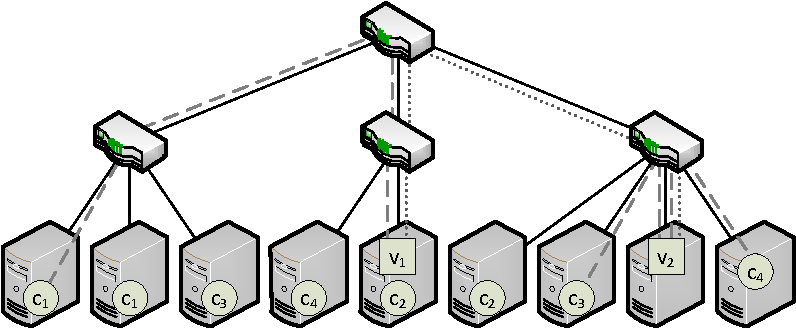
\includegraphics[width=0.79\columnwidth]{figs/static-mapping/data_locality_no_legend.pdf}
\caption{Overview: a 9-server datacenter storing~$\tau=4$ different chunks~$\{c_1,\ldots,c_4\}$ (depicted as \emph{circles}), each having two replicas. The replicas need to be selected and assigned to the two
 virtual machines~$v_1$ and~$v_2$; the virtual machines are depicted as \emph{squares}, and
 the network connecting them to chunks (using bandwidth~$\CostTrans$) is \emph{dashed}. In addition, the virtual machines are inter-connected among
 each other using bandwidth~$\CostCom$ (\emph{dotted}). The objective of the embedding algorithm is to minimize the overall bandwidth allocation.}\label{fig:overview}
\end{figure}


\parag{Optimization Objective.} 
Our goal is to design algoriths that minimize the resource \emph{footprint}, the most common objective function considered in the literature \cite{fischer-survey}.
Formally, let~$\dist(v,\achunk)$ denote the~distance (in the underlying physical network~$\Tree$) between a~node~$v$ and
its assigned (active) replica~$\achunk$, and let~$\dist(v_1,v_2)$ denote the distance between the two nodes~$v_1$ and~$v_2$.
We define the \emph{footprint}~$\Cost(v)$ of a node~$v$ as follows:
$$
\Cost(v) = \underbrace{\sum_{\achunk \mid \mu(c) = v} \CostTrans \cdot \dist(v,\achunk)}_{\text{chunk access cost}} +  \underbrace{\frac{1}{2} \cdot \sum_{v' \in \VirtualNodes\setminus\{v\}} \CostCom \cdot \dist(v,v')}_{\text{node inter-connect cost}},
$$
where~$\mu(v)$ is the set of chunks assigned to~$v$.
Our goal is to minimize the overall resource footprint $\Cost=\sum_{v\in V} \Cost(v)$.
The solution must obey the capacity of the substrate network: (1)~the total number of nodes hosted at each server $s$ must not excced $\capacity(s)$, and (2)~the total bandwidth allocated at each link $e$ must not exceed its capacity $\capacity(e)$.
%Finally, the solution must assign every chunk to some node, i.e. $\bigcup_v \mu(v) = \{ c_1, \ldots, c_{\tau} \}$.

\subsection{Problem Decomposition}

We introduced the $\CTE$ problem in its full generality.
To fully chart the algorithmic complexity of $\CTE$, we decompose the problem into its fundamental components that can be activated or deactivated independently of each other, and we consider all possible variants.
Concretely, we consider $5$ aspects of $\CTE$, namely multiple chunk assignment ($\MA$),
replica selection ($\RS$), flexible node placement ($\FP$), node inter-connect ($\NI$),
and bandwidth constraints ($\BW$), as~described in the following. 

\parag{Multiple Assignment ($\MA$).}
In most applications, the number of chunks~$\tau$ is larger than the number of nodes, and the objective is to assign multiple chunks to each node.
In each variant (regardless of $\MA$), we investigate assignments that balances chunks among nodes, i.e. where the number of chunks is divisible by the number of nodes, and each node processes an~identical integer number of chunks.
We require that the number of chunks processed by each node is equal to~$\MaFactor = \tau / n_V$, and we call $\MaFactor$ the multi-assignment factor.
If the number of chunks exceeds the number of nodes, i.e. $\MaFactor > 1$, then we refer to such scenario as $\MA$.
In~the~$\CTE$ variant without $\MA$, each node has exactly one chunk assigned, i.e. $\MaFactor = 1$.

\parag{Replica Selection ($\RS$).}
Distributed filesystems often utilize data redundancy for corruption detection and correction.
A redundant data chunk has multiple \emph{replicas}, stored on different physical machines.
For each data chunk, it is sufficient to process only one of its replicas.
By~$\RS$ we denote the flexibility of choosing which replica of each data chunk to process.
In~the~problem variant without $\RS$, each chunk has a single replica ($r_i = 1$ for all $i$).

\parag{Flexible Placement ($\FP$).}
%In most applications, nodes of virtual network are unconcerned about their physical placement.
By $\FP$ we denote the flexibility of assignment of nodes to~physical machines.
In the problem variant without $\FP$, the assignment of nodes to physical machines is given as an input.

\parag{Node Inter-Connect ($\NI$).}
In multiple computational tasks, it is sufficient to process data chunks independently of each other.
However, more often the result of processing the individual chunks is combined afterwards.
By $\NI$ we refer to the latter scenario, where the computation requires the nodes to cooperate.
We investigate the scenario, where we reserve a bandwidth of volume $\CostCom$ between each pair of nodes, i.e. the node inter-connect is modelled as a complete graph, to account for the all-to-all communication patterns of batch processing applications such as MapReduce.
In the problem variant without $\NI$, we optimize only the cost of transporting chunks to nodes, and the inter-node communication is set to zero, i.e. $\CostCom = 0$.

\parag{Bandwidth Capacities ($\BW$).}
We distinguish between an uncapacitated and a capacitated scenario where each link $e$
of the substrate network come with bandwidth
constraint $\capacity(e)$, and we refer to the bandwidth-constrained version by~$\BW$.
Note that capacity constraints introduce infeasible problem instances, where it is impossible to
allocate sufficient resources to~embed the virtual network.
In the problem variant without $\BW$, each link has infinite capacity, i.e. for each edge $e$, $\capacity(e) = \infty$.

\section{Polynomial-Time Algorithms}\label{sec:poly}


Despite the various degrees of freedom in terms of embedding and replica selection,
we can solve many problem variants efficiently.
 This section introduces three general techniques,
 which can roughly be categorized into
 \emph{flow} (Section~\ref{ssec:flow}), \emph{matching} (Section~\ref{ssec:match}) and \emph{dynamic programming}
 (Section~\ref{ssec:dyn}) approaches.
In Figure~\ref{fig:venn_full}, we either summarize the fastest method to solve the computational problem or its computational intractability.
 
First, let us make a simplifying observation:
\begin{obs}\label{obs:nofp}
In CTE variants without flexible placement (FP),
the bandwidth required
for the inter-connect network (NI) can be allocated upfront, 
as it
does not depend on the replica
selection and assignment.
Accordingly, we can reduce the variant~$RS+MA+NI+BW$ (as well as all its subproblems)
to~$RS+MA+BW$ (resp.~its subproblems).
\end{obs}

\begin{figure}[t]
\centering
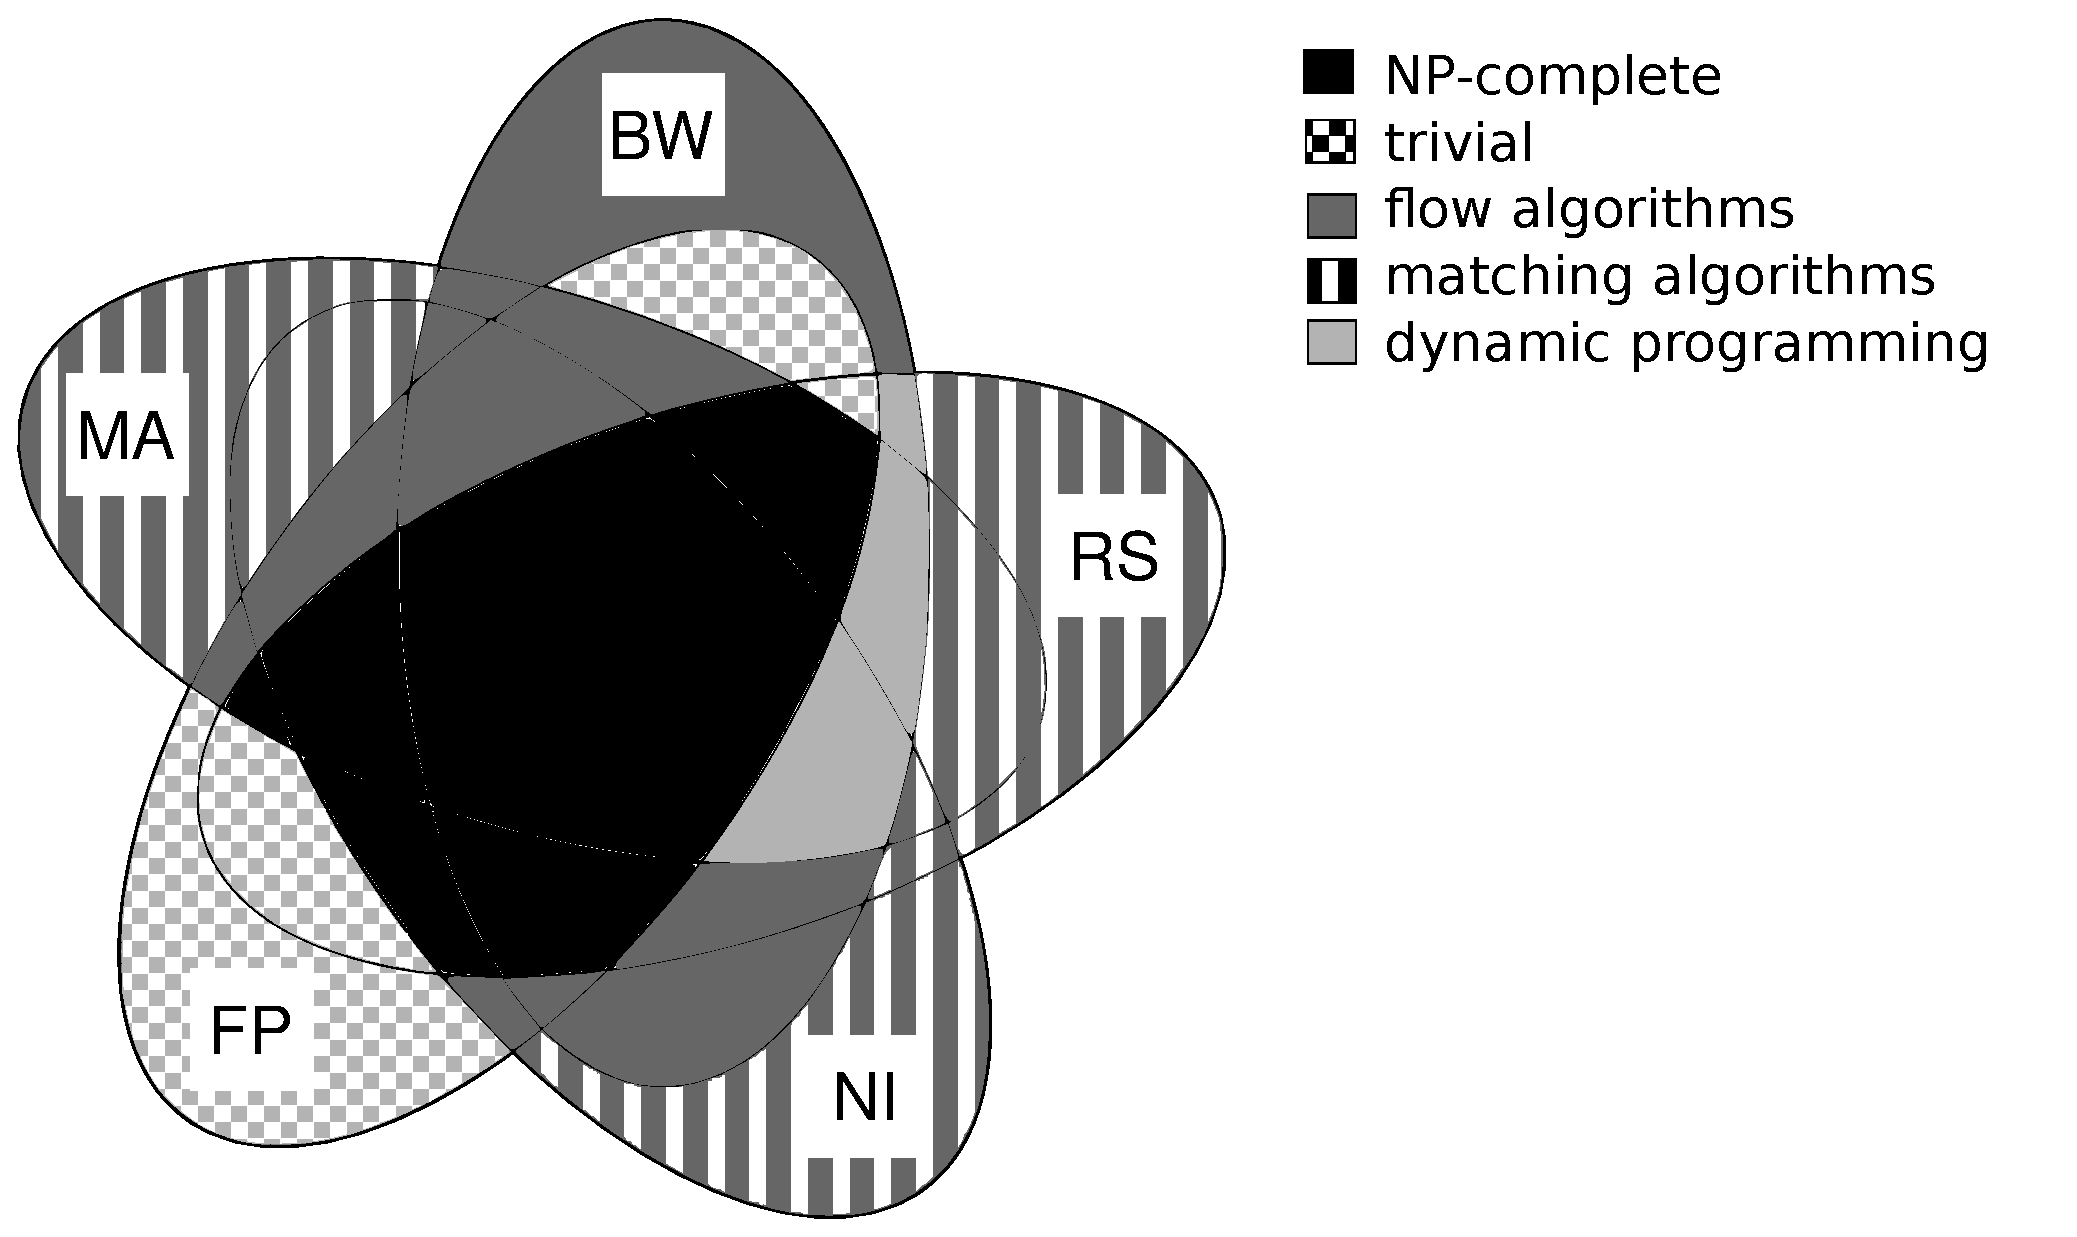
\includegraphics[width=0.69\columnwidth]{figs/static-mapping/venn_full2}
\caption{Fastest algorithms for different respective variants. Variants depicted by solid black are NP-hard, and variants depicted by checked filling are trivially solvable. For the remainder of variants we marked the fastest method.}
\label{fig:venn_full}
\end{figure}


\subsection{Flow-Based Algorithm}\label{ssec:flow}

\begin{figure}
\centering
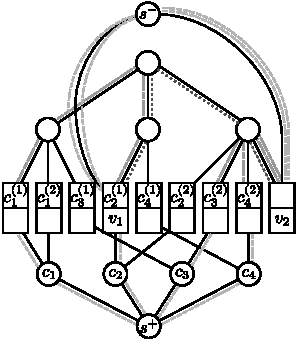
\includegraphics[width=0.5\columnwidth]{figs/static-mapping/flow_ma_cv}
\caption{An example of the extended substrate
network~$\Tree^*$: The sink~$\Sink$ is connected to the two leaves, which host the
nodes. The artificial nodes are depicted below the leaves, are labeled with
their respective chunks (e.g.,~$\achunk_1$), and are connected to the source
$\Source$ as well as to the leaves that contain replicas of their chunk.
The~maximum flow with minimum cost is indicated by the dashed lines: each line
represents one unit of flow. The~dotted lines indicate links which have reduced
capacity due to~$\NI$.}
%\caption{Example of flow construction: Problem instance with two nodes, four chunk
%types, and two replicas per type. The min-cost-max-flow
%is indicated by the dashed lines: each line represents one unit of flow.
%}
\label{fig:flow_construction}
\end{figure}



%\begin{figure}[t]
%\centering
%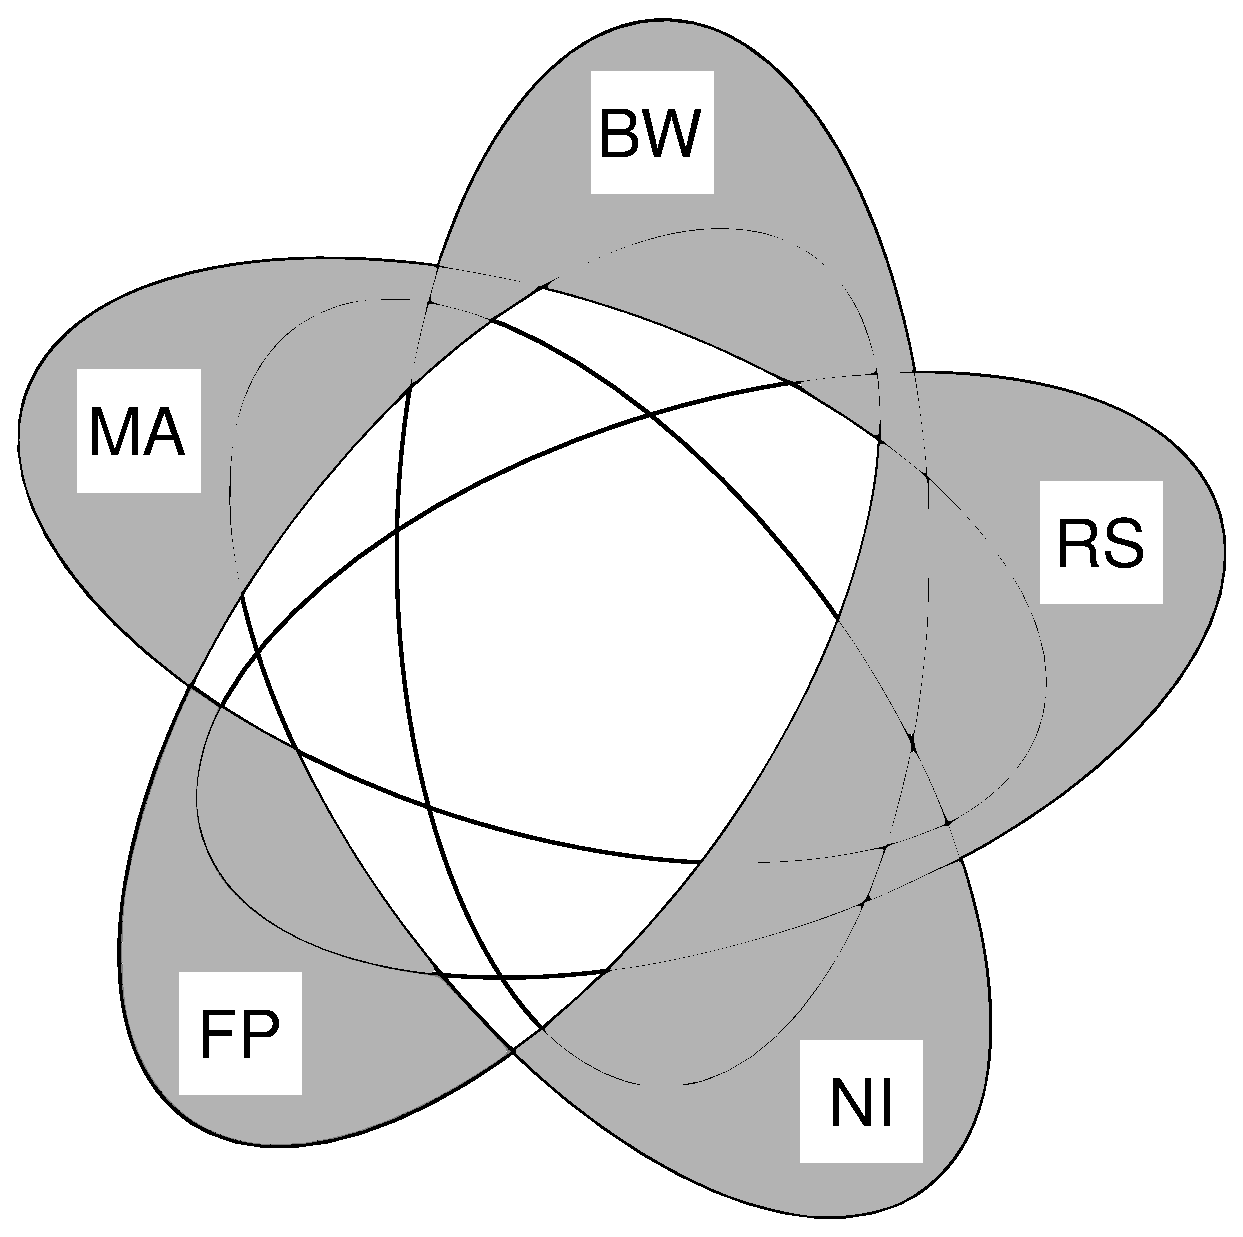
\includegraphics[width=0.49\columnwidth]{figs/static-mapping/venn_flow.pdf}
%\caption{Variants solved by flow approach.}
%\label{fig:venn_flow}
%\end{figure}


We first present an algorithm to solve the~$\RS+\MA+\NI+\BW$ variant of the $\CTE$ problem.
Recall that in this problem variant,
we are given a~set of redundant chunks ($\RS$) and a~set of
nodes
at fixed locations (no~$\FP$). The number of chunks may be larger than the number
of nodes ($\MA$), and each node needs to be connected
to its selected chunks as well as to other nodes ($\NI$), while respecting
capacity constraints ($\BW$).
As we see in the following, we can use a flow approach to solve this
problem variant.


\parag{Construction of the Artificial Graph.}
In order to solve the~$\RS+\MA+\NI+\BW$ variant of the {\CTE} problem,
we first remove the~$\NI$ component using Observation~\ref{obs:nofp}.
Then, we construct
an artificial graph~$\Tree^*$, extending the substrate network~$\Tree$.
We transform bandwidth capacities so that they correspond to the maximal number of chunks that we can transfer through the link.
Concretely, for~$\Tree^*$, for each link~$e\in E(\Tree)$, we set its new
capacity in~$\Tree^*$ to~$\lfloor\capacity(e) / \CostTrans\rfloor$.
After this normalization, we extend the topology~$\Tree$ by
introducing an artificial vertex for each of $\tau$ chunks. Each of these artificial
vertices is connected to each leaf (i.e., server) in~$\Tree$ where a replica
 of the respective chunk is located,
connecting the replica by a link of capacity~$1$. In
addition, we create a
\emph{super-source}~$\Source$, and connect it to each of the artificial chunk
vertices (with a link of capacity~$1$). Moreover, we create an artificial \emph{super-sink}~$\Sink$ and
connect it to every leaf containing at least one node; the link capacity represents
the number of nodes this server hosts times the~multi-assignment factor
$\MaFactor$.
We additionally assign the following costs to edges of~$\Tree^*$:
every edge of the original substrate network costs one unit, and all other artificial edges
cost nothing.
A solution to the~$\RS+\MA+\BW$ variant can now be computed
from a solution to the \emph{min-cost~max-flow} problem between super-source
$\Source$ and
super-sink~$\Sink$ on the artificial graph~$\Tree^*$.
An illustration of this construction is presented in Figure~\ref{fig:flow_construction}.

\parag{Algorithm.}
Our algorithm to solve the~$\RS+\MA+\NI+\BW$ variant consists of three parts:
First, we construct the normalized and extended graph~$\Tree^*$
described above and compute
a~min-cost-max-flow solution.
State-of-the-art min-cost-max-flow algorithm is the double scaling algorithm~\cite{mincostmaxflow-state}, which is based on the scaling technique~\cite{mincostmaxflow-1,mincostmaxflow-2}, .

Second, we have to \emph{round} the resulting, possibly fractional flow, to
integer values. Due~to the~\emph{integrality theorem}~\cite{flow-book},
there always exists an optimal integer solution on graphs with integer capacities.
However, min-cost~max-flow algorithms may yield fractional solutions
which need to be rounded to integral solutions (of the same cost)~\cite{electric-flows}.

Third, given an integer min-cost-max-flow solution, we need to decompose
the integer flow into the paths
representing matched chunk-node pairs:
The assignment can be obtained by decomposing the flow allocated in the
original substrate network. In order to identify a matched chunk-node pair,
we take an~arbitrary (loop-free) path~$p$ carrying a flow of value at least~$1$ from~$\Source$ to~$\Sink$:
the first hop represents the chosen chunk, the second hop the chosen
replica, and the penultimate hop represents the server: we assign
the replica to an arbitrary node on this server that has less than $\MaFactor$ chunks assigned.
Having found this pair, we reduce the flow
along the path~$p$ by one unit.
We continue the pairing process until every chunk is assigned.

\parag{Analysis.}
The runtime of our algorithm consists of four parts: construction of~$\Tree^*$,
computation of the min-cost-max-flow, flow rounding, and decomposition. The
dominant term in the~asymptotic runtime is the flow computation.
Using the double scaling algorithm for min-cost-max-flow~\cite{mincostmaxflow-state}, we get a runtime of~$\mathcal{O}(|E|^2 \cdot\log\log U \cdot \log |E|)$
where~$|E| = n_S+\sum_{i=1}^\tau r_i$ is the number of $\Tree^*$ edges, and~$U$ is the maximal link capacity. Note that in networks with high capacity
and uncapacitated networks, we can simply set~$U=\tau$, so the resulting overall runtime is $\mathcal{O}(|E|^2 \cdot\log\log \tau \cdot \log |E|)$


\subsection{Matching Algorithms}\label{ssec:match}


%\begin{figure}[t]
%\centering
%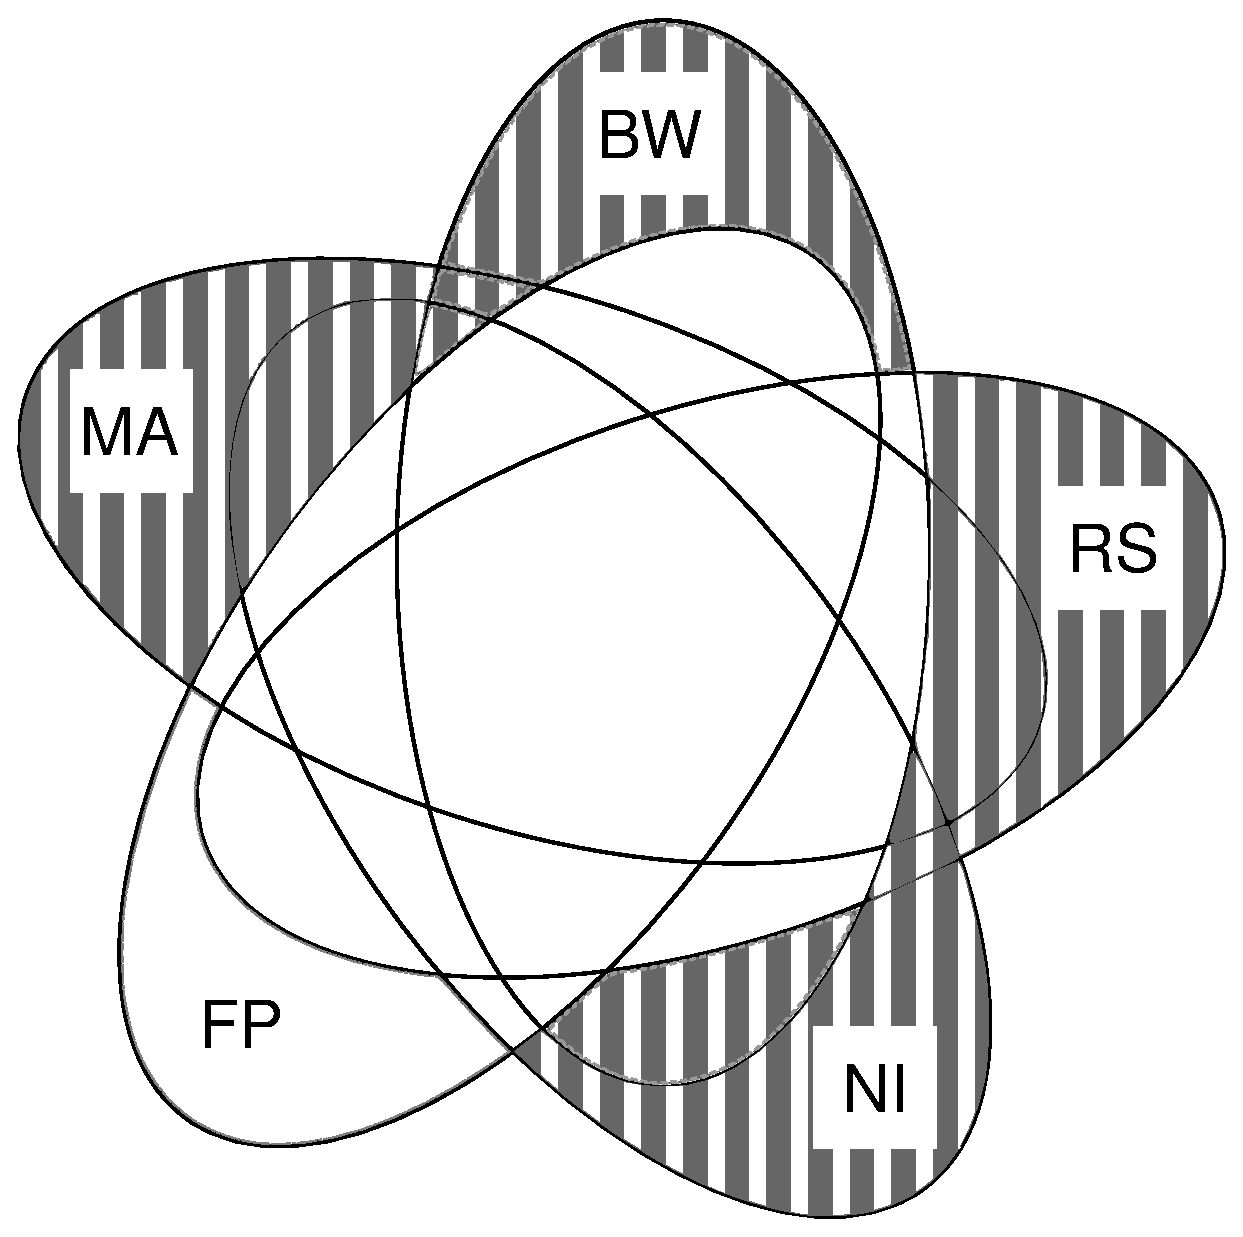
\includegraphics[width=0.49\columnwidth]{figs/static-mapping/venn_matching.pdf}
%\caption{Variants solved by matching approaches.}
%\label{fig:venn_match}
%\end{figure}
This section presents faster algorithms to solve 
two variants of $\CTE$ problem, $\RS+\MA+\NI$ and~$\MA+\NI+\BW$, that can also be solved with the flow approach
introduced above.
First, we consider the~$\RS+\MA+\NI$ variant.
Recall that in this variant,
we are given a~set of redundant chunks ($\RS$) and a~set of nodes
at fixed locations (no $\FP$). The number of~chunks may be larger than the number
of nodes ($\MA$), and each node needs to be connected
to its chunks as well as to other nodes ($\NI$).

\parag{Algorithm.} Due to Observation~\ref{obs:nofp}, the $\RS+\MA+\NI$ variant degenerates to~$\RS+\MA$.
In order to solve the latter,
we construct a bipartite
graph between the set
$\VirtualNodes$ of nodes and
the set of chunks.
First, we clone each node~$\MaFactor$ times,
as each node needs to process
$\MaFactor$ chunks, and we aggregate all replicas of a given chunk in a
single %$\ChunkType$
super-vertex.
Second, we link (cloned) nodes to (aggregated) replicas.
In instances without $\BW$, mapping of any replica to any node is feasible, and hence, for a given mapping of chunks to nodes $\mu$, the minimum bandwidth is utilized if for each $c$, node $\mu(c)$ serves the closest replica of $c$.
Therefore, for each node $v$ and chunk $c$, we connect $v$ and super-vertex $c$ with the link of cost $\min_i \dist(v,c^{(i)})$, i.e., the cost of reaching the closest replica.
Finally, on the resulting bipartite graph, we compute a~\emph{minimum weight
perfect
matching}:
the resulting matching describes the optimal assignment of chunks to nodes.
An example instance is presented in Figure~\ref{fig:matching}.


\begin{figure}
  \centering
  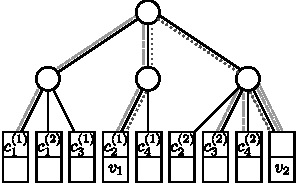
\includegraphics[width = 0.39\columnwidth]{figs/static-mapping/model_ma_r_cv_boxes}
  \centering
  \hspace{1cm}
  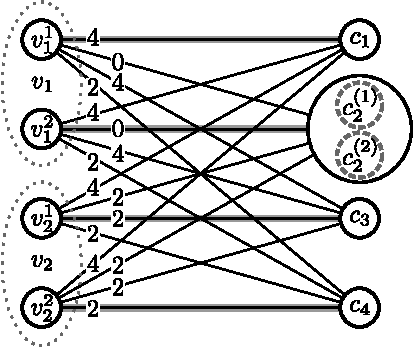
\includegraphics[width =0.39\columnwidth]{figs/static-mapping/matching}
\caption{The~$\RS+\MA$ variant on the \emph{left} is converted into a
  matching problem instance on the \emph{right}.
The figure illustrates
an instance where two nodes are
cloned into~$\MaFactor = 2$ nodes each,
resulting in a total of four nodes in
the matching representation.
The two replicas of each chunk are
aggregated into a single chunk vertex~$\achunk_j$  in the matching instance;
this gives a total of four chunk vertices in the matching graph. The costs
on the links between all clones of a specific vertex and a chunk are set to
the minimum distance. We can observe this for instance at the edges connecting
the two clones of~$\VirtualNode_1$ to~$\achunk_2$: both weights are 0.
}
\label{fig:matching}
\end{figure}

\parag{Analysis.}
The runtime consists of two parts: the construction of the matching graph and
the~actual matching computation. The constructed graph consists of
$\MaFactor \cdot (n_V \cdot \ChunkType) = \tau^2$
many edges,
and for each edge we compute its weight. The shortest distances
in a tree can be computed in time~$\mathcal{O}(t + q)$~\cite{offline-lca}, where $t$ is the size of a tree and $q$ is the number of queried pairs, which translates to the overall construction time~$\mathcal{O}(n_s + n_v\cdot \sum_{i=1}^\tau r_i)$.
The state-of-the-art algorithm to compute matchings~\cite{matching-best} has a running time of $\tilde{\mathcal{O}}(|E|^{10/7}\cdot \log W)$, where $|E|$ is the number of edges, $W$ is the maximum weight of an edge, and $\tilde{\mathcal{O}}$ hides polylogarithmic (in terms of $|E|$) factors.
The total running time is then $\tilde{\mathcal{O}}(\tau^{20/7}\cdot \log(n_s)) + \mathcal{O}(n_v\cdot \sum_{i=1}^\tau r_i)$.
The matching-based algorithm outperforms the flow-based algorithm.


\subsubsection{Local matching algorithm}

In this section, we present the way to solve the~$\MA+\NI$ variant even faster by exploiting
locality. Moreover, we show that we can
even solve
$\MA+\NI+\BW$ variants by simply
verifying feasibility.
In~the~following, due to Observation~\ref{obs:nofp}, we can focus on
the~$\MA$ and~$\MA+\BW$ variants, respectively.
We start by lower-bounding the required bandwidth allocation.
The \emph{uplink} of a subtree $T$, denoted $\Uplink(T)$ is an edge from the root of the subtree to its parent.

%We first introduce the following definition.
%\begin{defn}[Local Assignment (LA)]\label{def:loc}
%We define an assignment~$\VmChunkAssignment$ to
%be \emph{local in a specific subtree~$\Tree'$}, iff~$\VmChunkAssignment$
%assigns the maximum number of chunks in the
%subtree to nodes in the same subtree.
%We define~$\VmChunkAssignment$ to be \emph{local} when
%it is local with respect to all possible subtrees of the~substrate network.
%\end{defn}
%
%\begin{figure}
%\center
%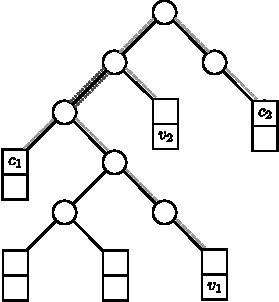
\includegraphics[width = 0.45\columnwidth]{figs/static-mapping/unbalanced_tree}
%\caption{Illustration of local assignment: The dashed lines indicate bandwidth allocations, which occur
%independently of the chosen assignment. The dotted lines indicate bandwidth
%allocation which occur only if~$c_2$ is assigned to~$v_1$.}
%\label{fig:unbalanced_tree}
%\end{figure}
%
%\parag{Example.}
%Figure \ref{fig:unbalanced_tree} illustrates the concept of local assignment:
%The closest chunk to~$v_2$ is~$c_1$, and the closest node to~$c_1$ is~$v_2$.
%However, a subtree~$T'$ exists such that~$v_1 \in T'$ and~$c_1
%\in T'$, but~$v_2 \notin T'$. Therefore, a local assignment cannot assign~$c_1$ to~$v_2$.


%Later we will see that
%optimal solutions to
%$\MA$ have a local assignment. We exploit this in our algorithms described
%in the following.


\begin{lemma}\label{lem:uplink-alloc}
Given the~$\MA$ variant and a subtree~$\Tree'$
containing~$x$
chunks and~$y$ nodes, the bandwidth allocation of any
assignment
$\VmChunkAssignment$ on the uplink of~$\Tree'$ is at~least $|x-y\cdot\MaFactor|\cdot
\CostTrans$.
\label{lemma:uplink}
\end{lemma}
\begin{proof}
In case the number of chunks equals the processing capacities of the
nodes in the given subtree,
the bandwidth allocation inflicted by the chunk access network on the uplink can
be
zero, since we can assign all chunks to nodes in the same subtree.
Otherwise, we distinguish between two cases. If there are more chunks in the subtree, at least all of the excess chunks have to
be transferred to a different subtree, which 
inflicts costs~$\CostTrans$ per excess chunk on the uplink connecting~$\Tree'$
with the
remaining parts of~$\Tree$.
 Similar situation occurs if the processing capabilities exceed the
amount of
available chunks.
Hence, the minimum bandwidth allocation for the chunk access on the uplink
is the absolute difference between the number of chunks and the processing capabilities
of the subtree, i.e.~$|x-y\cdot\MaFactor|$ times $\CostTrans$, the amount of bandwidth needed
for a single transfer.
\end{proof}


\parag{Algorithm.} Our proposed algorithm for the $\MA$ variant of $\CTE$
proceeds in a bottom-up fashion, traversing the~substrate network~$\Tree$
from the leaves toward the root.
For each subtree~$\Tree'$, we maintain
two sets~$S_c,S_v$ in order to match unmatched
chunks~$S_c$ in the subtree~$\Tree'$ to unmatched
nodes~$S_v$ in~$\Tree'$. Both sets are initially empty.
We associate a counter with each node that enters $S_v$, and we intitialize it to $\MaFactor$, the multi-assignment factor.


We first process all the leaves, in an arbitrary order; subsequently, we process arbitrary inner vertices
of~$\Tree$ whenever all their children have been processed.
We process any leaf~$\ell$
by adding any
nodes or chunks which are located on~$\ell$ to the corresponding sets~$S_c$ and~$S_v$.
A non-leaf vertex~$u$ is processed in the following way: we take the union of
the sets of~$u$'s children, i.e., the sets contain the unmatched chunks and nodes
in this subtree.
For both leaves and inner nodes, whenever
both sets are non-empty, we greedily match an arbitrary chunk $c$ in~$S_c$ with an arbitrary node $v$ in~$S_v$.
Then, we remove $c$ from $S_c$, and we decrement the counter of $v$. If the counter of $v$ reaches zero, we remove $v$ from $S_v$.

\parag{Analysis.} For each
vertex in the substrate graph,
we build the union of the
children's sets,
and since each vertex can only be the child of one vertex,
the amortized runtime per vertex is constant.
The number of all remove operations is equal to
the number of chunks~$\mathcal{O}(\ChunkType)$.
Hence the overall complexity of this construction amounts to
$\mathcal{O}(n_S + \ChunkType)$.
The local matching algorithm outperforms the previous algorithm that relied upon calculating the minimum-weight perfect matching.

%It remains to prove optimality of such local assignments.
%By \emph{uplink} of a subtree with root $r$ we denote the edge from $parent(r)$ to $r$ (if it exists).
%We first characterize the bandwidth allocation on uplinks of subtrees.

%\begin{theorem}
%Given an~$\MA+\NI$ variant instance, a feasible assignment~$\VmChunkAssignment$
%is optimal iff it is local.
%\label{thm:local_optimal}
%\end{theorem}
%
%\begin{proof}
%Local assignments generate exactly the minimal allocations on all links, as
% the assignments which generate the minimal bandwidth allocations
%described in
%the proof of
%Lemma~\ref{lemma:uplink} are local in the given subtree. Hence
%each local assignment has to be optimal. A non-local assignment, has at least
%one subtree, in which it is not local. This subtree has a higher
%allocation on the uplink. Since the local assignment has minimal allocations
%on all other links, the non local assignment has a larger footprint.
%\end{proof}

The algorithm allocates the minimum possible bandwidth at an uplink of every subtree, as stated in Lemma~\ref{lemma:uplink}, and hence the algorithm is optimal.
Combined with a simple postprocessing step, this approach can also solve~$\MA+\BW$ variant. The central idea of this extension is
that \emph{local} assignments allocate the minimal bandwidth
on each individual edge. In consequence, each bandwidth constraint,
which is lower than the allocation of a local assignment on one link, renders
the problem infeasible. Hence, it is sufficient to temporarily omit the
bandwidth limitations, compute an optimal assignment for an~$\MA$ instance, and
verify that the resulting allocations do not violate any capacities. The
postprocessing step scales linearly with the number of edges in the substrate
graph.


\subsection{Dynamic Programming}\label{ssec:dyn}

We now show how to solve the~$\MA+\FP+\NI+\BW$ variant
in polynomial time.
Note that this variant requires to find a
tradeoff between the desire to place nodes as close as possible to each other
(in order to minimize communication costs), and the desire to place nodes
as close as possible to
the chunk locations.




\parag{Example.} Figure~\ref{fig:dynamic_motivation} shows an example: one
extreme solution is to minimize the distance between chunks and nodes,
see mapping~$\NodeMapping_1$ in the left picture in
Figure~\ref{fig:dynamic_motivation}: the four nodes are all
collocated with chunks, resulting in a zero-cost chunk access network. As a
result, the paths between the individual nodes are longer than in alternative
node placements: each node has a distance of two hops to one other node,
and four hops to two other nodes. Hence the resulting allocations for the
node inter-connect sum up to~$20 \cdot \CostCom$.

%\begin{figure}[t]
%\centering
%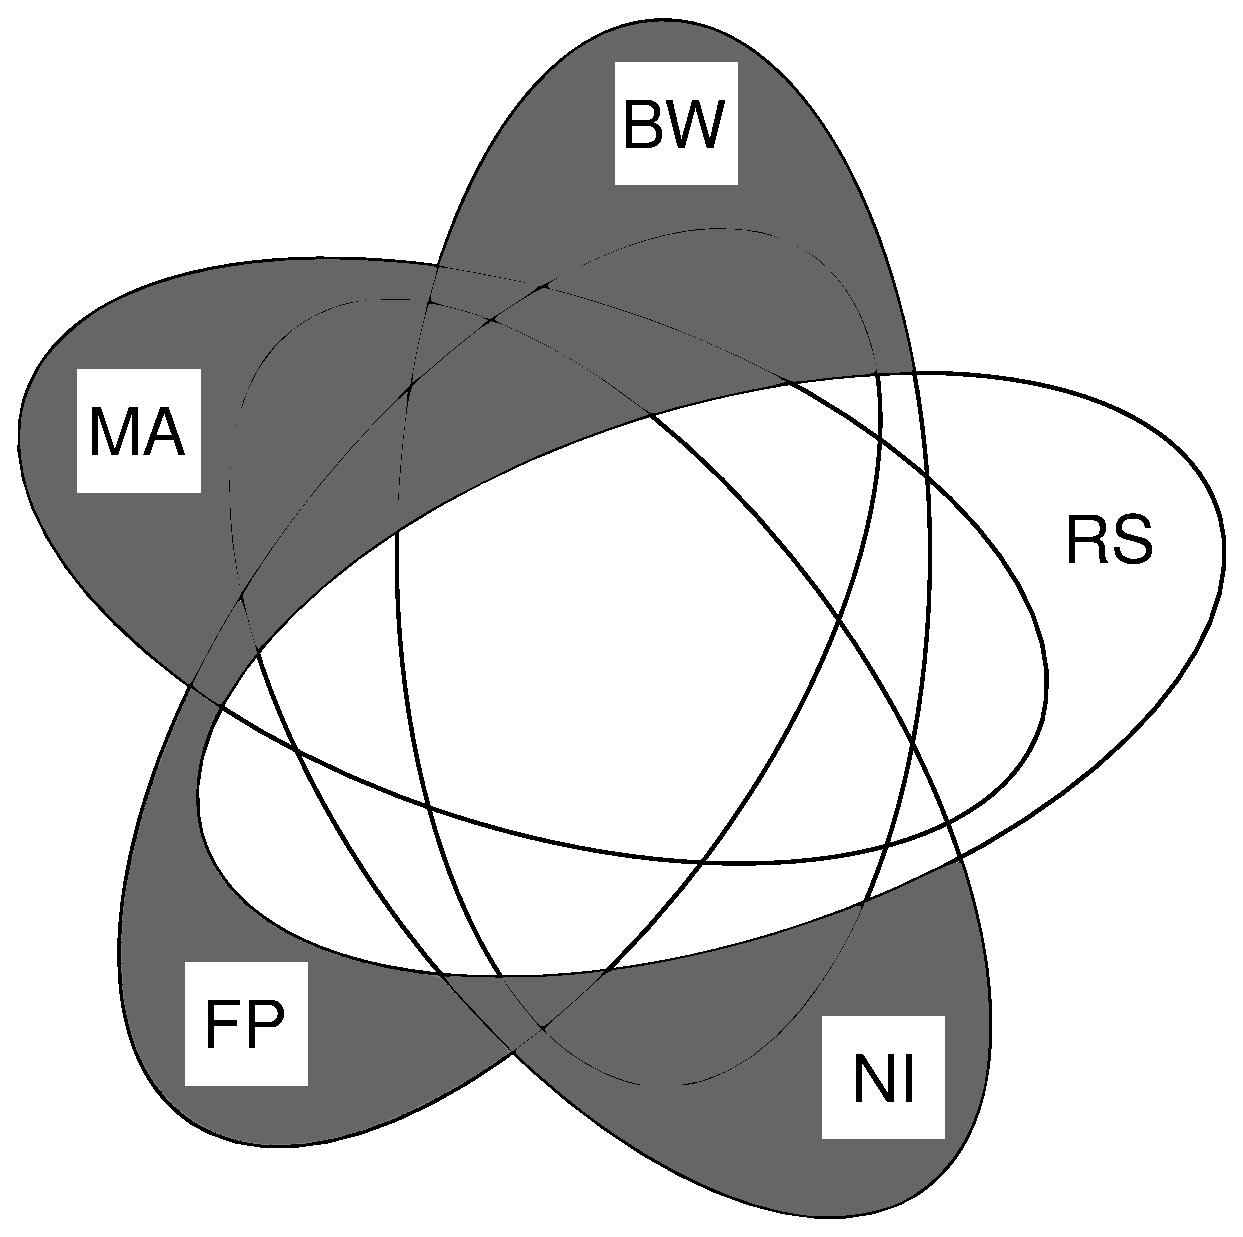
\includegraphics[width=0.49\columnwidth]{figs/static-mapping/venn_dp.pdf}
%\caption{Variants solved by dynamic programming approach.}
%\vspace{-1em}
%\label{fig:venn_dp}
%\end{figure}

The right picture in Figure~\ref{fig:dynamic_motivation} shows a different node
mapping~$\NodeMapping_2$, which seeks to minimize the communication costs
between the nodes, and places all nodes in one subtree. The distance between all
nodes is two, which results in a total bandwidth allocation of~$12\cdot\CostCom$
for the inter-connect. However, this reduced price comes at additional costs in
the access network:~$c_3$ and~$c_4$ have to be communicated to~$v_3$ and~$v_4$,
which requires a total bandwidth allocation of~$8 \cdot \CostTrans$.


\begin{figure}
  \centering
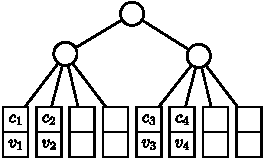
\includegraphics[width = 0.39\columnwidth]{figs/static-mapping/dynamic_bad}
\hspace{1cm}
\centering
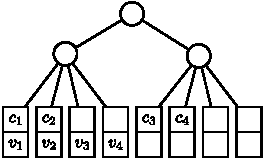
\includegraphics[width = 0.39\columnwidth]{figs/static-mapping/dynamic_good}
\caption{Two different node placements for the same substrate graph and chunk
locations. For~$\CostTrans = \CostCom$, both solutions have an identical
footprint. In other cases, one solution outperforms the other.}
\label{fig:dynamic_motivation}
\vspace{-1em}
\end{figure}



\parag{Algorithm.} Our proposed approach is based on dynamic programming, and
leverages the \emph{optimal substructure property} of the $\MA+\FP+\NI+\BW$ variant:
as we will see, optimal solutions for subtrees
can be efficiently combined into optimal solutions for the whole tree.
For ease of presentation, we transform the
substrate network~$\Tree$
into a binary tree:
we clone every higher-degree node,
iteratively attaching additional clones as right children
and original children as left descendants.
New edges between cloned vertices constructed during the binarization have infinite capacity.

As usual in dynamic programs, we define, over the structure of the tree, a
recursive formula~$f$ for
the minimal cost solution given any possible number of nodes
embedded in a given subtree (the actual set of nodes does not matter,
due to symmetry).
The value of $f(T, x)$ corresponds to the bandwidth cost of placing $x$ nodes in a subtree $T$.
The total bandwidth cost consists of the bandwidth allocated inside $T$, and the bandwidth conducted outside of $T$.
The formula to calculate the fuction $f$ for a subtree containing only a leaf $\{ \ell \}$ is the following:
\[
f(\{ \ell \}, x) =
\begin{cases}
   \infty & \mbox{if } x > cap(\ell)\enspace,\\
   \infty & \mbox{if } bw(\{ \ell \}, x) > cap(\Uplink(\ell))\enspace,\\
    bw(\{ \ell \}, x) & \mbox{otherwise}\enspace, \\
  \end{cases}
  \]
where $bw(T,x) := \CostTrans \cdot |x - \ChunkCount(T)| +\CostCom \cdot
(\Vms - x) \cdot x$, and $\ChunkCount(T)$ is the number of chunks in a~subtree~$T$.
The first term of $bw$ represents the required bandwidth for the communication between the~$x$
nodes inside~$T$, and the~$\Vms - x$ nodes in the remaining parts of the substrate
network.
The second term represents
the bandwidth necessary to transport the chunks in $T$ from their location to
nodes outside of $T$ (see Lemma~\ref{lemma:uplink} for similar argument).
We set~$f(\{ l \},x)$ to infinity if the required bandwidth
$bw$ exceeds the capacity~$\capacity$ of the uplink of~$\{ l \}$, or $x$ exceeds the node hosting capacity of server $l$.


The formula to calculate the fuction $f$ for a non-leaf subtree $T$ is the following:
\[
  f(T, x) = 
    \min_{0\leq r \leq x} \{  f\left(\textsc{Le}(T),
x-r\right) +
f\left(\textsc{Ri}(T), r\right) \} + bw(T,x)
  \]
To calculate the value of $f$ for non-leaf subtries, we split the~$x$ nodes
into two positive integer
values, and we put~$r$ on the right and~$x - r$ on the left subtree.
That is, we take the optimal cost
(given recursively) of placing~$r$ nodes in
the right subtree~$\textsc{Ri}(T')$ of~$T'$ and~$x-r$ nodes in left subtree~$\textsc{Le}(T')$ of
$T'$. Given the cheapest combination, we add the bandwidth requirements
on the uplink of~$T'$ to generate the overall costs for placing~$x$ nodes in~$T'$.
Therefore,~$f(T',x) =   \min_{0\leq r \leq x}$~$ \{  f\left(\textsc{Le}(T'),
x-r\right) +$~$
f\left(\textsc{Ri}(T'), r\right) \} + bw(T',x)$.
Again, we set~$f(T',x)$ to infinity if the required bandwidth
$bw$ exceeds the capacity~$\capacity$ of the uplink of~$T'$.

We compute~$f$ in a bottom-up manner. 
To finally compute the actual optimal embedding,
we traverse the computed minimal-cost path backwards,
according to
the optimal values found for~$f$ during the bottom-up computation.


\parag{Analysis.}
The substructure optimality follows from the observation that
costs can be accounted on the uplink, and the fact
 that we check each possible node distribution.
For each substrate vertex ($n_S$ many) we have
to check the cost of all possible splits,
resulting in an overall complexity of~$\mathcal{O}(n_S \cdot n_V^2)$.
The runtime to binarize~$\Tree$ is asymptotically negligible in comparison.


\subsection{Simple Variants}

%\begin{figure}
%\centering
%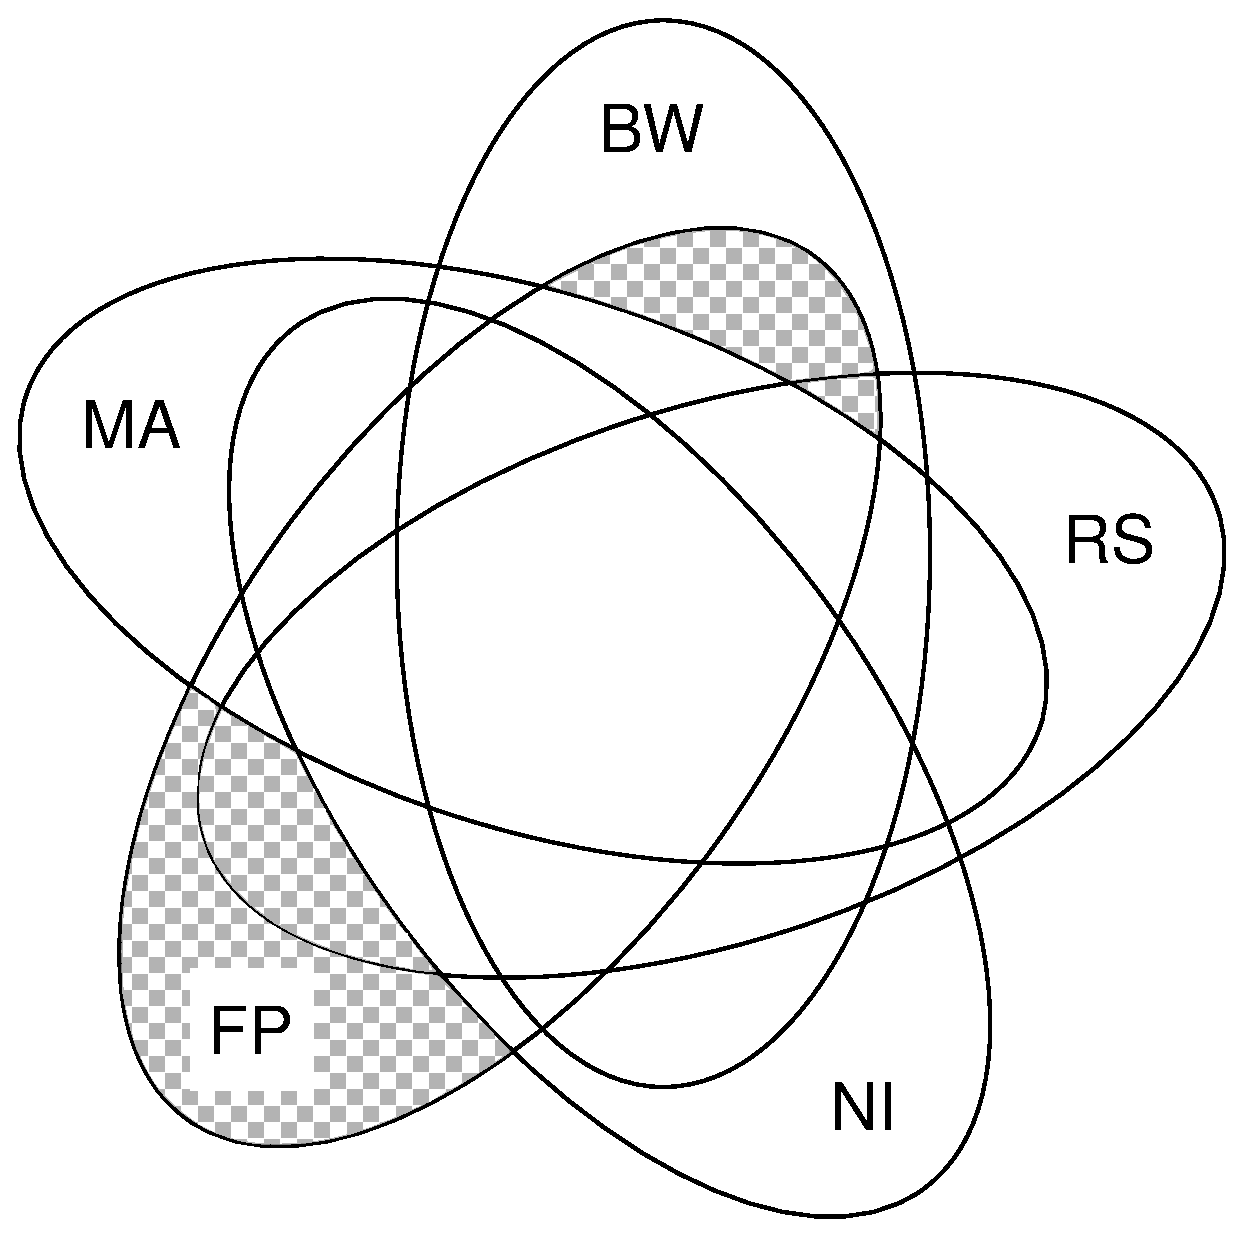
\includegraphics[width=0.49\textwidth]{figs/static-mapping/venn_trivial.pdf}
%\caption{Trivially solvable variants.}
%\label{fig:venn_trivial}
%\end{figure}


For the sake of completeness, we also observe that there are
several variants that admit a trivial solution. Concretely, variants with~$\FP$
plus any combination of
$\RS$ and~$\BW$ (but without~$\MA$ and~$\NI$) can easily be solved by
mapping
nodes to chunk locations.
%Figure~\ref{fig:venn_trivial}
%shows a Venn diagram of the trivial property combinations.

%%%%%%%%%%%%%%%%%%%%%%%%%%%%%%%%%%%%%
\section{NP-Hardness Results}\label{sec:np}

We have seen that even variants with multiple dimensions of
flexibility can be solved optimally in polynomial time.
This section now points out fundamental
limitations in terms of computational tractability.
In particular, we
show that variants become NP-hard if flexibly placeable nodes ($\FP$) have to be assigned to one of multiple replicas ($\RS$), either with multiple chunks per node ($\MA$ in Section~\ref{ssec:fprsma}) or with communication among nodes ($\NI$ in Section~\ref{ssec:fprscc}).
Both results hold even in uncapacitated networks, and even in small-diameter
substrate networks (namely two- or three-level trees).
The hardness of variants $\FP+\RS+\MA$ and~$\FP+\RS+\NI$ imply
the hardness of four additional, more general variants.

In addition to hardness results for aforementioned $\CTE$ variants, we study the influence of restricting number of replicas of a chunk on computational tractability on those variants.
Namely, we introduce the restricted replica selection component $\RS(r_{max})$, parametrized by an integer $r_{max}$, that restricts the number of replicas of any chunk: for every chunk $c_i$ we have $r_i < r_{max}$.
We consider $\RS(2)$ component in relation with Multi-Assignment ($\MA$) and Node-Interconnect ($\NI$).
Concretely, in Section~\ref{ssec:fprsma} we first present the NP-hardness of unrestricted scenario $\FP+\RS+\MA$ (Theorem~\ref{th:ma-unlimited}) as a warm-up,
and then we present more refined hardness result for $\FP+\RS(2)+\MA$ (Theorem~\ref{th:ma-reduction}). In Section~\ref{ssec:fprscc} we present the NP-hardness of unrestricted scenario $\FP+\RS+\NI$ (Theorem~\ref{theorem:fp_rs_cc}).
However, restricted replica selection $\RS(2)$ in combination with Node-Interconnect required additional ways to control the placement of nodes, and the NP-hardness result uses bandwidth constraints $\BW$.

\subsection{Introduction to 3D Perfect Matching}
\label{sec:3dm_intro}

Both the hardness of~$\FP+\RS+\MA$ and~$\FP+\RS+\NI$ variants of the $\CTE$ problem are shown by a reduction
from the NP-complete problem of \emph{3D Perfect Matching}~\cite{3dmatch},
which can be seen as a generalization of bipartite matchings to 3-uniform
hypergraphs. We refer to this problem by~$\TDM$, and for completeness,
review it quickly:
$\TDM$ is defined as follows. We are given three finite and disjoint
sets~$X$,~$Y$, and~$Z$ of cardinality~$k$, as well as a~subset of triples~$P\subseteq
X \times Y \times Z$.  Set~$M \subseteq P$ is a 3-dimensional matching
if and only if, for any two distinct triples~$t_1=(x_1, y_1, z_1) \in M$
and~$t_2=(x_2, y_2, z_2) \in M$, it holds that~$x_1\neq x_2$,~$y_1\neq
y_2$, and~$z_1\neq z_2$. Our goal is to decide if we can construct
a~$M \subseteq P$ which is \emph{perfect}, that is, a~subset which covers all
elements of~$X \cup Y \cup Z$ exactly once.


\subsection{Hardness of Multi-Assignments}\label{ssec:fprsma}

\subsubsection{Warm-up: Multi-Assignment with Unrestricted Number of Replicas}

Our proof that the variant $\FP+\RS+\MA$ of the $\CTE$ problem is NP-hard is based on the following construction.
Let~$I$ be an instance of~$\TDM$ with $p$ triples and set cardinality $k$ (where $k = |X| = |Y| = |Z|$).
We construct an instance~$\ICTE$ of the $\CTE$ problem in the following way:
\begin{itemize}
\item \emph{Tree construction:} We create a tree consisting of a root,
and for each triple from $P$, we create a \emph{triple gadget} which we directly attach as
a child of the root. The gadget is of height 2,
and consists of an inner node and three leaves.
\item \emph{Chunks:} For each element in~$X$,~$Y$ and~$Z$,
 we create a chunk
($3 \cdot k$ chunks in total). Every gadget contains three chunk replicas (one per leaf),
corresponding to the elements of the triple.
\item \emph{Other properties:} We set the number of to-be-embedded nodes $n_V = k$,
$\CostTrans = 1$, and the the multi-assignment factor
$\MaFactor=3$.
\item \emph{Threshold.} In order to turn the optimization problem into a decision problem, we use
a cost threshold~$\Thr = 4\cdot k$. The cost threshold is met by all
assignments which assign all three chunks of each triple gadget to a
node which is collocated with one of the chunks. Assignments which connect a
chunk to a node in a different triple have a larger footprint, and are
considered to be infeasible.

\end{itemize}

%\parag{Example.} Figure~\ref{fig:fprsma} shows an example of our construction: In an~instance~$\ITDPM$
%of 3-DM sets $X, Y, Z$ consist of the following elements: $X = \{ x_1, x_2 \}, Y = \{ y_1, y_2 \}$ and $Z = \{ z_1, z_2 \}$.
%Set of triples $P$ contains three triples
%$(x_1, y_1,
%z_1)$,~$(x_2, y_1, z_2)$, and~$(x_2, y_2, z_2)$. This instance has only one solution:~$M =
%\{(x_1,y_1,z_1),(x_2,y_2,z_2))\}$.
%
%To construct the corresponding instance~$\ICTE$ of the $\CTE$ problem, we
%create a gadget for each triple in~$P$. For each variable which occurs in a
%triple, the corresponding gadget contains a~chunk of the
%type of the variable. The triple
%$(x_2, y_1, z_2)$ of the instance is represented by the middle gadget in
%Figure~\ref{fig:fprsma}. The objective of~$\ICTE$ is to allocate~$k=2$ nodes
%with the smallest possible footprint. If the total footprint is at most $4\cdot k$, we can construct a solution to~$\ITDPM$ from the solution to~$\ICTE$.
%The footprint consists of the costs which occur when a node is embedded in a~gadget, and the three chunks of that gadget which are assigned to that node: one of
%the chunks is collocated with the node, the other two have to be transferred
%via two hops, incurring unit costs on each hop.

Figure~\ref{fig:fprsma} shows an example of our construction.

\begin{figure}[t]
  \centering
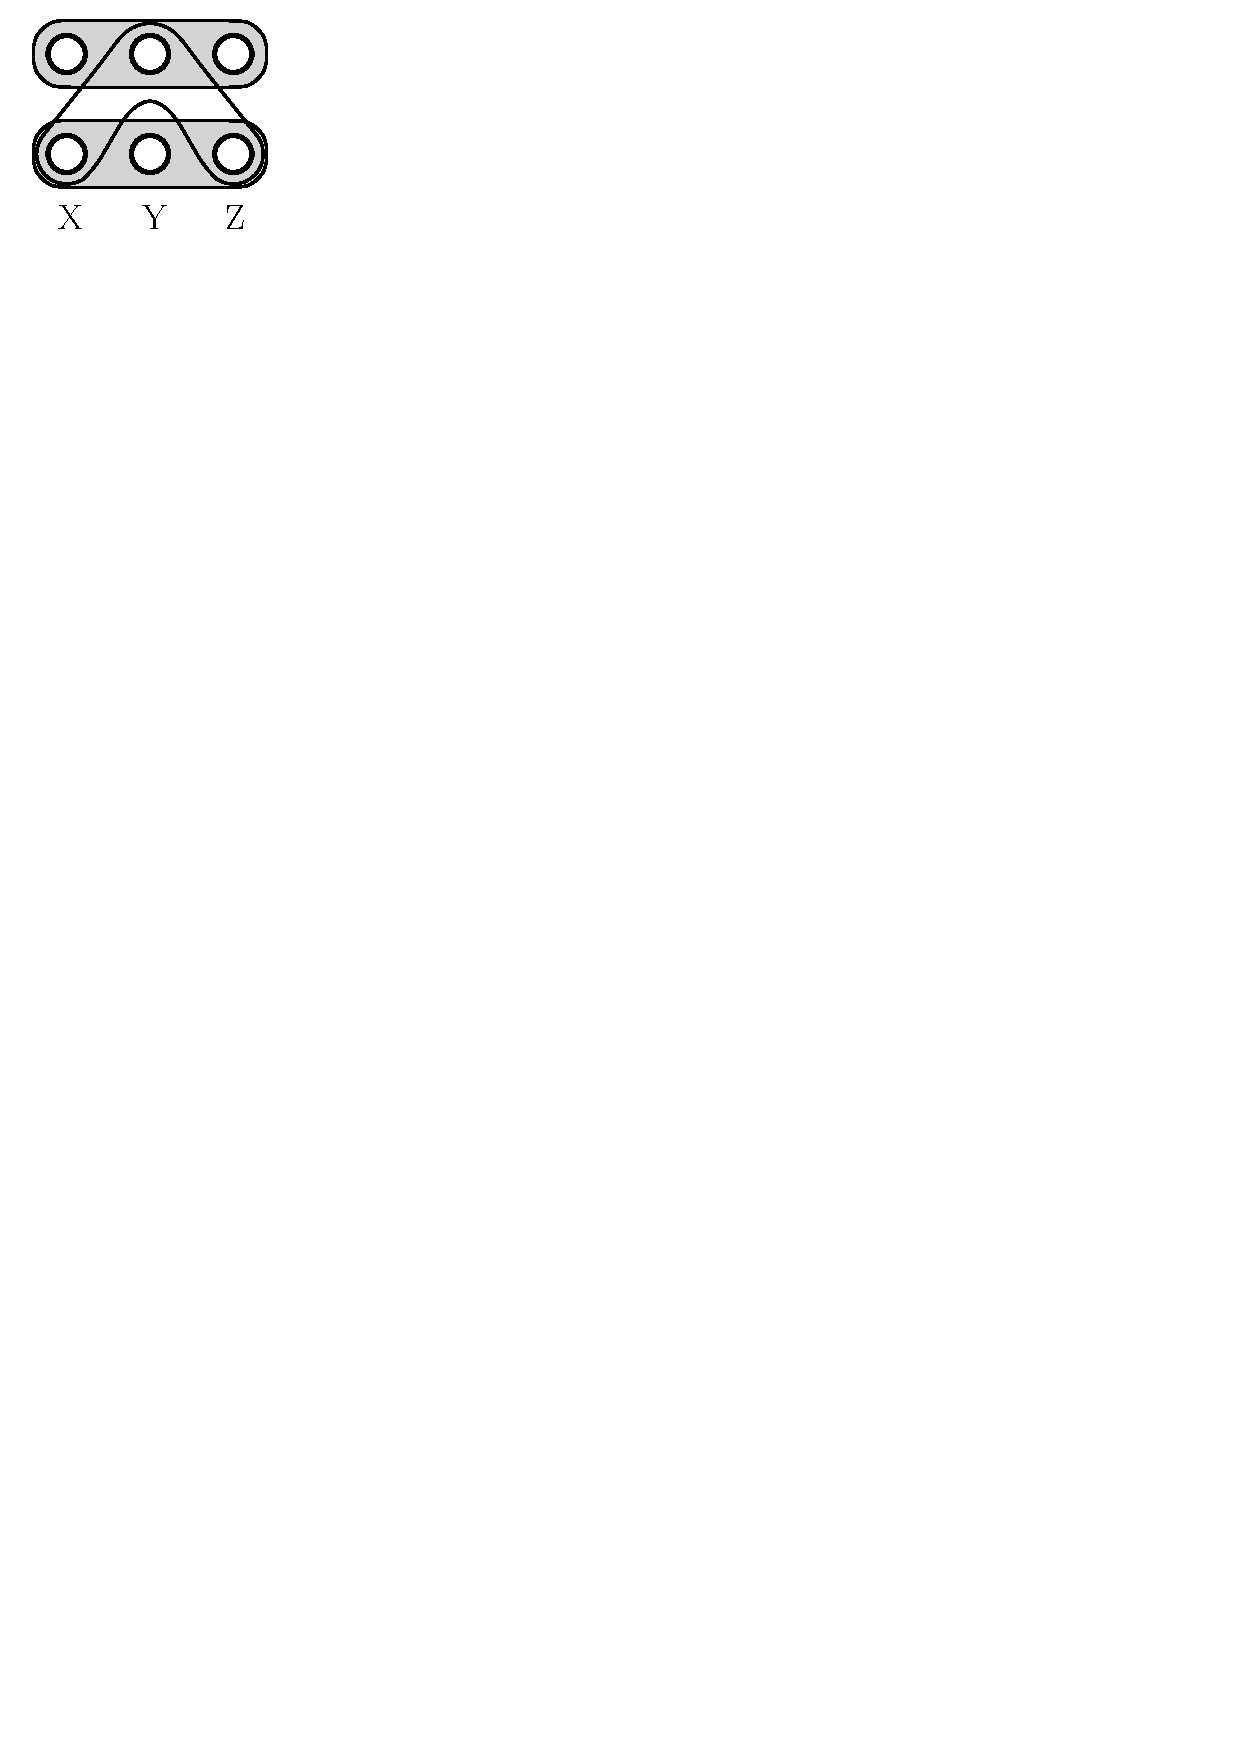
\includegraphics[width = 0.21\columnwidth]{figs/static-mapping/tdm-horizontal}
\hspace{1cm}
\centering
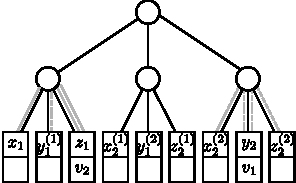
\includegraphics[width = 0.4\columnwidth]{figs/static-mapping/np_3dm_construction}
\hfill
\caption{\textit{Left:} A~$\TDM$ instance of cardinality $k=2$ with three triples:
$(x_1, y_1, z_1)$,~$(x_2, y_1, z_2)$, and~$(x_2, y_2, z_2)$. The solution is
indicated by the grey triples. \textit{Right:} The corresponding instance and an optimal solution for the~$\FP + \MA
+ \RS$ of the $\CTE$ problem. Each triple corresponds to a single triple gadget.}
\hfill
\label{fig:fprsma}
\end{figure}


\parag{Correctness.}
Given these concepts, we can now show the computational hardness.
\begin{theorem}
  Variant $\FP+\RS+\MA$ of the $\CTE$ problem is NP-hard.
  \label{th:ma-unlimited}
\end{theorem}
\begin{proof}
Let~$\ITDPM$ be an instance of~$\TDM$ and let~$\ICTE$ be an instance of
the~$\FP+\RS+\MA$ variant constructed as described above. We prove that~$\ICTE$ has a solution of cost at most $\Thr = 4 \cdot k$ if ($\Rightarrow$) and only if
($\Leftarrow$)
$\ITDPM$ has a~perfect matching (of size~$k$).

($\Rightarrow$) Fix a feasible solution for~$\ITDPM$. We place a single node in every
gadget that corresponds to the chosen triples (of arbitrary leaf of this gadget). In each of the corresponding
gadgets, we match every chunk to the node in this gadget. This
solution has
cost exactly~$\Thr = 4\cdot k$: each of $k$ nodes processes $1$ chunk collocated with it, and $2$ chunks at the distance $2$. As every element of the universe is covered, every
chunk is processed.

($\Leftarrow$) Fix a solution for ~$\ICTE$ of cost at most $\Thr$.
We call the triple gadget \emph{active} if it hosts a node in one of its leaves.
To construct the solution to $\ITDPM$, we pick triples, whose gadgets are active.
Now, we claim that in each triple gadget there is at most one node.
As every leaf hosts at most one chunk, hence each node can process at most $1$ of its $\MaFactor=3$ chunks for free.
Hence, each node incurs the cost at least $4$ for the remaining $2$ chunks that are at distance at least $2$.
Assume that two nodes $n_1$, $n_2$ are placed in the same triple gadget.
As a triple gadget contains $3$ chunks, at least $2$ of $6$ chunks that they process are placed outside of this triple gadget.
Hence, $n_1$ and $n_2$ incur a cost at least $4$ to reach each of those exterior chunks.
In total, $n_1$ and $n_2$ incur a cost at least $12$, and the total cost $4\cdot k + 4$ exceeds the threshold $\Thr = 4\cdot k$.
Therefore, exactly $k$ gadgets are active, and the solution to $\ITDPM$ consists of $k$ triples.
Since all chunks are processed, every element of~$X$,~$Y$ and~$Z$ is matched.
\end{proof}

\subsubsection{Mult-Assignment with at most 2 replicas}

We have seen that replica selection flexibility can render embeddings computationally hard.
Now, we provide a more detailed look at this hardness result
and explore the minimal requirements for rendering replica selection hard.
In particular, we show that already two replicas for each chunk are sufficient for computational intractability.

% We now show that the 2-replica selection variant is even NP-hard
%without capacity constraints.  In particular, we consider the 
%variant~$\RS(2)+\MA(4)+\FP$ with at most two replicas of each chunk and assignment factor
%four. There are no capacity constraints on links.
%
%Our construction consists of two major modifications to hardness result without replication factor restrictions (for that result, refer to Section~\ref{ssec:fprsma}).
%
%\parag{Unique chunks on the comb.} First, we provide the tools for restricting the placement of nodes in certain parts of the tree.
%In Section~\ref{ssec:fprsma}, due to symmetric structure of the tree, the carefully crafted threshold value allowed us to prove that e.g. no Triple Gadget ever had two or more nodes placed in it.
%We still use the threshold value as the placement mechanism, but in this section, due to the asymmetrical tree construction, we combine it with the concept of unique chunks on the comb (by \emph{comb} we denote the balanced tree, where all non-root vertices have at most one child).
%
%For an introduction to the concept of unique chunks, let us consider the following example.
%Suppose that within one $\VCEMB$ construction, we would like to encode not one $\TDPM$ instance, but two $\TDPM$ instances: $M_1$ and $M_2$, with disjoint universe and different number of triples to be chosen: $n_1$ and $n_2$.
%We perform the following modifications to the encoding provided in Section~\ref{ssec:fprsma}.
%The multi-assignment factor grows by $1$, that is the instance we construct is the $\RS+\MA(4)+\FP$ variant instance.
%We construct two subtrees $T_1$ and $T_2$, that correspond to $M_1$, resp. $M_2$; we construct two two-edge-level combs $C_1$ and $C_2$, with number of leaves $n_1$, resp. $n_2$.
%We attach $M_1$ and $C_1$ (resp. $M_2$ and $C_2$) to the common root and we name the resulting subtree $P_1$, resp. $P_2$.
%Next, we attach $P_1$ and $P_2$ to the common root.
%In the end, the height of the tree grew by $2$.
%Finally, we populate both combs with unique chunks, and we set the number of to-be-placed nodes to $\Vms = n_1+n_2$.
%We modify the threshold to be the sum of the thresholds for constructions for $M_1$ and $M_2$ plus $4\cdot (n_1 + n_2)$.
%The last substrate of the threshold value corresponds to transportation of the fourth chunk processed by each machine for the distance of four.
%
%To see why the example indeed can solve two instances of $\TDPM$, we need the following observations.
%First, we claim that no node is ever placed in a comb.
%To prove this fact, we use the property of the comb that the leaves are highly separated, and the fact that each machine has to process $4$ chunks.
%Next, we claim that the number of nodes placed in $P_1$ (resp. $P_2$) is $n_1$ (resp. $n_2$).
%To see this, consider any imbalance of the number of placed nodes; notice that some chunks in the underpopulated comb are processed outside of their $P_i$ subtree, resulting in the solution that exceeds the threshold.
%
%\parag{Families of chunks.} The second tool that we introduce allows us to express the redundancy of chunks without actually replicating chunks more than two-fold.
%For simplicity of introduction, we consider the scenario with no multi-assignment.
%For each chunk $c$ with redundancy, we count the number of occurrences of replicas of such a chunk in the tree, and name it $r_c$.
%We replace the chunk $c$ with $r$ chunks, which we call the family $F_c$ of that chunk.
%For each occurrence of replica of $c$, we replace it with a replica of any chunk from the family (without repetitions).
%To this point, the redundancy factor was reduced from $r_c$ to $1$.
%Now, we construct the gadget $G_c$ for chunk $c$, which consists of $r_c$ leaves, each hosting the second replica of each chunk from family $F_c$.
%We use the technique of unique chunks on the comb to constraint the number of nodes in $G_c$ to be exactly $r_c - 1$.
%We provide necessary additional $r_c-1$ nodes to be placed.
%Hence, exactly $1$ node is placed on a chunk of family $F_c$ outside the gadget $G_c$, and exactly $r_c-1$ nodes cover the remaining $r_c-1$ chunks inside gadget $G_c$.
%All chunks are processed, the replication factor is reduced to $2$, and the size of construction grows polynomially.

%\parag{Introduction to the reduction.} As we already stated, we modify the construction from Section~\ref{ssec:fprsma}.
%As a way to deal with replication, we use the families of chunks using the unique chunks on the comb.
%We extend the construction of a gadget for chunk with redundancy, by incorporating the fact that the multi-assignment factor is $4$.
%For the construction to remain correct given such a multi-assignment factor, we introduce further chunks with one chunk replica to place in the chunk gadget and use the excessive $3$ data processing capacities.

\parag{Construction.} For an arbitrary instance~$\ITDPM$ of the~$\TDM$ problem we construct a~$\RS(2)+\MA+\FP$ variant instance~$\IVCEMB$ the following way.
Let $k = |X|=|Y|=|Z|$ and $p = |P|$.
For each $e\in X\cup Y\cup Z$, by $P_e$ we denote the set of all triples that contain element $e$.
Let $\deg(e) = |P_e|$, and note that $\sum_e \deg(e) = 3\cdot |P|$.
We proceed with the construction as follows.

\paragraph{Tree.}
We construct the tree that has the following structure (see Figure~\ref{fig:red-ma2}):

\begin{figure}[t]
  \centering
  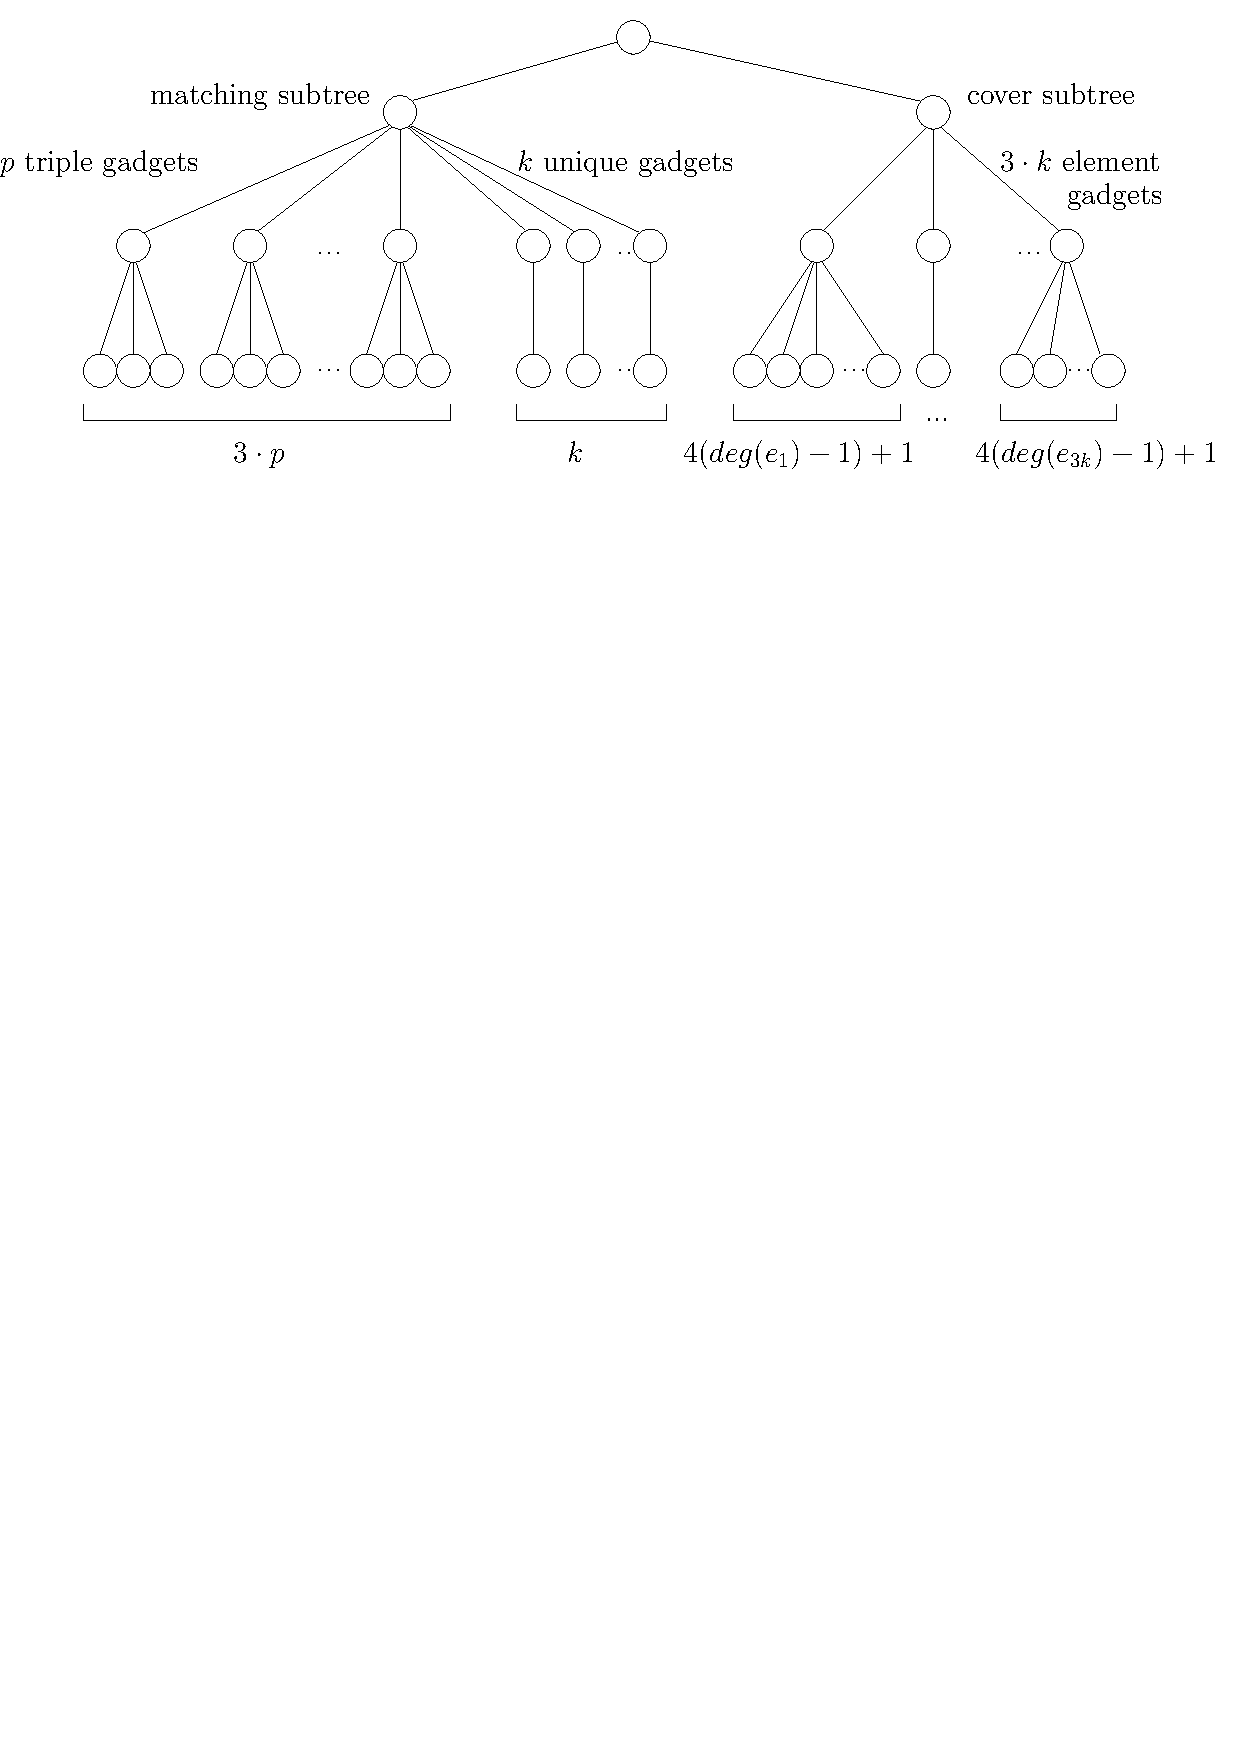
\includegraphics[width=0.9\columnwidth]{figs/static-mapping/overview}
  \caption{Overview of the substrate network.}
  \label{fig:red-ma2}
\end{figure}

\begin{enumerate}
  \item The physical network consists of two subtrees connected to the
  root: the \emph{\MatchSubtree} and the \emph{\CoverSubtree}. The
  {\MatchSubtree} consists of $p$ \emph{\TripleGadgets}, one per each triple from $P$ and $k$
  \emph{\UnqGadgets}. The {\CoverSubtree} consist of~$3\cdot k$ {\ElGadgets}, one for each element $e\in X\cup Y\cup Z$.
  \item The {\TripleGadget} consists of four vertices: three leaves and the root of the gadget, as defined in the previous reduction in this section.
  \item The {\UnqGadget} consists of two vertices: the leaf and the root of the gadget.
  This keeps the tree balanced, and it also keeps leaves of
  {\UnqGadgets} far from each other.
  \item The {\ElGadget} for element $e$ consists of the
  root and~$4\cdot(\deg(e)-1)+1$ leaves.
\end{enumerate}

\paragraph{Chunks.}
We construct three sets of chunks.
The first set corresponds to elements of the universe (that is, $X\cup Y\cup Z$).
The construction of such chunks is similar to construction of chunks in Section~\ref{ssec:fprsma}, but to take into consideration the restricted replication factor, we change the construction.
Namely, for each element of universe $e \in X \cup Y \cup Z$, we construct $\deg(e)$ chunks, each having exactly two replicas.
The other two sets of chunks has one replica, therefore those are called \emph{unique} chunks.
We construct two types of unique chunks, distinguished by a different role in the construction.
For unique chunks we simply identify the chunk with chunk replica.
\begin{enumerate}
  \item For each triple $t \in P$, we construct $3$ chunks:~$c(t \cap X, t), c(t \cap Y, t), c(t \cap Z, t)$.
  Each chunk $c(e, t)$ has two replicas: $c^{(1)}(e,t)$ and $c^{(2)}(e,t)$.
  In total we construct $6\cdot p = 2\cdot \sum_e\deg(e)$ chunk replicas that we put in the matching subtree.
  In the {\TripleGadget} for triple $t$ we put
  three replicas:
 ~$c^{(1)}(t \cap X, t), c^{(1)}(t \cap Y, t), c^{(1)}(t \cap Z, t)$, one per each leaf.
  \item We construct~$k$ additional chunks named
  ~$u_1, \ldots, u_k$ with one replica each, and we place those at the leaves of \UnqGadgets (one chunk per leaf).
  \item For each element~$e\in X\cup Y\cup Z$,
  we construct additional~$3\cdot(\deg(e) - 1)$ chunks, with one replica each.
  We call this set~$\UniqueE$.
\end{enumerate}
Those chunks are placed in the following parts of the tree:
\begin{enumerate}
  \item \emph{Chunks in the Matching Subtree:} In {\TripleGadget} of triple $t$ we put
  three replicas:
 ~$c^{(1)}(t \cap X, t), c^{(1)}(t \cap Y, t), c^{(1)}(t \cap Z, t)$, one per each leaf.
  \item \emph{Chunks in the Unique Gadgets:} We place replicas
 ~$u_1,\ldots, u_k$ at the leaves of \UnqGadgets.
 \item \emph{Chunks in Element Gadgets:} Consider the \ElGadget{} for the element $e \in X\cup Y\cup Z$.
 We place two types of replicas in the leaves of the gadget.
 We put replicas $c^{(2)}(t, e)$ for each $t \in P_e$.
 Additionally, we place all the replicas from set $\UniqueE$.
 In total, we place $4\cdot (\deg(e) - 1) + 1$ replicas, one per each leaf of the gadget.
\end{enumerate}

\paragraph{Other properties of the instance.}
\begin{enumerate}
  \item \emph{Multiple assignment:} We set the multi-assignment factor to $m=4$.
  \item \emph{Number of nodes:} We set the number of nodes to embed to
 ~$\numNodes = k + \sum_{e}(\deg(e)-1) = 3\cdot p - 2\cdot k$.
 \item \emph{Threshold:} We set the following threshold:
 ~$\Thr = 18\cdot p - 10\cdot k$.
 This value corresponds to the cost of solution, where $k$ nodes are matched to $4$ chunks that are in distance: $0, 2, 2$ and $4$ to the node, and remaining $\Vms-k$ nodes are matched to $4$ chunks that are in distance: $0, 2, 2$ and $2$ to the node.
\end{enumerate}

\parag{The reduction.}
Given any $\TDPM$ instance $\ITDPM$, we produce corresponding instance $\IVCEMB$ of the $\RS(2)+\MA+\FP$ variant, in the way described above.

The reduction (Theorem~\ref{th:ma-reduction}) unfolds in two stages.
First, given a solution $\STDPM$ to $\ITDPM$, we construct a solution $\SVCEMB$ to $\IVCEMB$.
This part is the easier of the two, and mainly consists of placing nodes in Triple Gadgets for triples chosen in $\STDPM$.

In the second stage, given $\SVCEMB$, we construct the $\STDPM$.
In this stage, the main difficulty lies in showing that $\SVCEMB$ has certain structure.

We call the {\TripleGadget} \textit{active}, if it contains a node at any leaf, and we call the node \textit{active} if it is placed in {\TripleGadget}.
Our goal is to show that in every feasible solution, exactly $k$ \TripleGadgets{} are active (Lemma~\ref{lem:n-active-ma}), and hence we can construct $\STDPM$ from the triples that correspond to active \TripleGadgets{} in $\SVCEMB$.

In $\IVCEMB$, chunks can be matched to nodes at distance $0, 2, 4$ or $6$.
  We call the matches at distance $0$ the \emph{free matches}, the matches at distance $2$ the \emph{neighbouring matches}.
  In addition we call the matches at distance $0$ or $2$ the \emph{short matches}, and the matches at distance $4$ or $6$ the \emph{long matches}.
  We call the distance between the pair of leaves the \emph{short distance}, if the distance between them is at most $2$, otherwise we call said distance the \emph{long distance}.

Proving the existance of more than $k$ long matches is sufficient to show that the instance is infeasible, as its cost exceeds the threshold.
To see this, note that the threshold value $\Thr$ corresponds to the cost of solution, where $k$ nodes has $1$ free match, $2$ neighbouring matches and $1$ long match at distance of $4$ hops, and remaining $\Vms-k$ nodes has $1$ free match and $3$ neighbouring matches assigned.
Note that the limit of $\Vms$ free matches is exhausted, hence excessive long matches cannot be compensated in any way.
Hence, at most $k$ long matches are present in any feasible solution.


\begin{lemma}
  In $\SVCEMB$ there are have exactly $k$ nodes placed in the \MatchSubtree.
  \label{lem:n-matchsubtree-ma}
\end{lemma}

\begin{proof}
 We claim that each node placed in the \MatchSubtree{} results in at least one long match.
This fact is a consequence of the structure of the tree and the fact that multi-assignment factor is set to $4$.
For each node placed in the \MatchSubtree{}, by the construction of the tree, the node has at most $3$ leaves in short distance, hence at least one of the matches is long.
Hence, we conclude that placing more than $k$ nodes in the \MatchSubtree{} results in more than $k$ long matches, which results in infeasibility of the solution.
In addition, each node placed in \UnqGadget{} results in at least $3$ long matches, as the only leaf in short distance is the leaf collocated with the node.

At most $k$ nodes are placed in \MatchSubtree{}, hence at least $\Vms-k$ nodes are placed in the \CoverSubtree.
Assume then that $\Vms-k+i$ nodes were placed in the \CoverSubtree{} for non-negative $i$.
Now, we argue that such node configuration results in $3\cdot i$ long matches.
Consider the \ElGadget{} $g_e$ for element $e$.
The gadget $g_e$ has exactly $4\cdot(\deg(e)-1)+1$ leaves, each hosting exactly one chunk replica.
As $4\cdot(\deg(e)-1)+1 \mod 4 = 1$, placing $\deg(e)-1+j$ nodes in $g_e$ for non-negative $j$ results in at least $3\cdot j$ long matches by the fact that there are insufficient chunk replicas in the short distance.
Using the fact that $\sum_e(\deg(e)-1) = 3\cdot p - 3\cdot k = \Vms - k$, by pidgeon-hole principle we conclude that indeed placing $\Vms-k+i$ nodes in the \CoverSubtree{} results in at least $3\cdot i$ long matches.

Consider the configuration with $\Vms-k+i$ nodes were placed in the \CoverSubtree{}, and $k-i$ nodes were placed in the \MatchSubtree{}.
Such configuration results in at least $2\cdot i + k$ long matches, where $3\cdot i$ long matches come from the excessive nodes were placed in the \CoverSubtree{}, and $k-i$ long matches come from $k-i$ nodes in the \MatchSubtree{}.
Hence we deduce that $i = 0$, as otherwise the number of long matches would exceed $k$.

\end{proof}

\begin{lemma}
  In $\SVCEMB$ no node were placed in \UnqGadget{}.
  \label{lem:no-unq-ma}
\end{lemma}
\begin{proof}
  By Lemma~\ref{lem:n-matchsubtree-ma}, exactly $k$ nodes were placed in the \MatchSubtree{}.
Suppose that out of $k$ nodes in the \MatchSubtree{}, a non-negative number of nodes $j$ were placed in the \UnqGadgets{}.
From the fact that each leaf of \UnqGadget{} has long distance to every other leaf, every node placed in \UnqGadget{} result in at least $3$ long matches.
Hence, the total number of long matches is at least $k-j + 3\cdot j$.
Finally, for the solution to be feasible we allow at most $k$ long matches, therefore no node was placed in the \UnqGadget{}.
\end{proof}

\begin{lemma}
  In $\SVCEMB$ there are have exactly $k$ active \TripleGadgets{}.
  \label{lem:n-active-ma}
\end{lemma}
\begin{proof}
  By Lemmas~\ref{lem:no-unq-ma} and \ref{lem:n-matchsubtree-ma} we conclude that $k$ nodes was placed in the \TripleGadgets.
As there are exactly $3$ replicas in each \TripleGadget{}, placing more than one node in a single \TripleGadget{} results in at least additional $3$ long matches.
Hence, exactly $k$ \TripleGadgets{} are active.
\end{proof}

\begin{lemma}
  In $\SVCEMB$ every chunk replica besides $u_1, \ldots, u_k$ is matched by a short match.
  \label{lem:short-ma}
\end{lemma}
\begin{proof}
  By Lemma~\ref{lem:n-active-ma}, exactly $k$ nodes are placed in \TripleGadgets{}, and by Lemma~\ref{lem:no-unq-ma} we deduce that chunks $u_1, \ldots, u_k$ are matched by long matches.
  As at most $k$ long matches are allowed for the solution to be feasible, remaining matches are short.
\end{proof}

\begin{theorem}
  The $\RS(2)+\MA+\FP$ variant of the $\CTE$ problem is NP-hard.
  \label{th:ma-reduction}
\end{theorem}

\begin{proof}
  
  Fix an instance $\ITDPM$ of~$\TDPM$.
  We show that~$\IVCEMB$ has a solution of cost~$\leq \Thr$ if and only if~$\ITDPM \in \TDPM$ (there exists a perfect 3D matching in $\ITDPM$).

  ($\Leftarrow$) Fix a feasible solution~$\STDPM$ for $\ITDPM$.
  We construct a solution~$\SVCEMB$ in the following way:
  \begin{enumerate}
    \item We place~$k$ nodes in~$k$ {\TripleGadgets} (one per gadget) that correspond to triples in~$\STDPM$.
    The choice of exact leaf of the gadget to place a node is arbitrary.
    We match each such node to $3$ chunk replicas in the gadget it is placed, and we match $1$ arbitrary, unmatched chunk replica in {\UnqSubtree}.
    \item In each {\ElGadget} that corresponds to element~$e$, we place
   ~$\deg(e) - 1$ nodes and match them to arbitrary chunks in this
    gadget, which are not yet matched in any {\TripleGadget}.
  \end{enumerate}

  We can observe that every chunk was processed, exactly $k + \sum_e(\deg(e) - 1)$ nodes are placed, and each of the nodes process exactly $4$ chunk replicas.
  To see that indeed the produced solution do not exceed the threshold $\Thr$, we sum up the total transportation cost.
  The $k$ nodes placed in \TripleGadgets{} have $1$ free match and $2$ neighbouring matches to chunk replicas within the \TripleGadget{}, and $1$ long match of cost $4$ (to some \UnqGadget{}).
  The remaining $\Vms-k$ nodes placed in the \CoverSubtree{} have $1$ free match and $3$ neighbouring matches.
  In total, the cost incurred is $8\cdot k + 6\cdot (\Vms - k) = \Thr$.
  Hence, the solution is indeed feasible.

  ($\Rightarrow$) Fix a feasible solution~$\SVCEMB$ for~$\IVCEMB$ in the way described in the construction section.
  By Lemma~\ref{lem:n-active-ma}, exactly $k$ \TripleGadgets{} are active.
  We construct the solution $\STDPM$ from the set of triples that correspond to active \TripleGadgets{}.

  It remains to show that $\STDPM$ indeed matches every element of $X\cup Y\cup Z$.
  By Lemma~\ref{lem:short-ma}, each match of $ch(e, t)$ for each $e\in X\cup Y\cup Z$ and each $t \in P$ is matched by a short match.
  Hence, each active node processes the 3 chunks that are placed in its \TripleGadget.
  In each {\ElGadget} for element~$e$, one chunk $ch(e, t)$ for some $t \in P$ is not matched.
  Let's call this chunk instance~$\Unmatched(e)$, and let's call~$\Unmatched = \cup_e \Unmatched(e)$.
  Note that~$|\Unmatched| = 3\cdot k$.
  The set~$\Unmatched$ is covered by \ActiveNodes{}, and hence the set of triples in $\STDPM$ form a 3D Perfect Matching of $X\cup Y\cup Z$.
\end{proof}



\subsection{Hardness of Inter-connects}\label{ssec:fprscc}


\subsubsection{Warm-up: Inter-connects with Unrestricted Number of Replicas}

Next, we prove that the joint optimization of node placement and replica selection
is NP-hard if an inter-connect has to be established between nodes.
In our terminology, this is the~$\FP+\RS+\NI$ variant.

The proof is similar in spirit to the proof of the~$\FP+\RS+\MA$ variant, however,
we modify the construction to account for the absence of~$\MA$:
we choose
a high value for~$\CostTrans$ (the cost of chunk transportation), such that nodes are directly collocated with
their assigned chunks. We leverage the fact that any solution which does not
assign 0 or 3 chunks to each gadget, has higher communication costs.

\parag{Construction.}
Let~$\ITDPM$ be an instance of~$\TDM$ with $p$ triples and set cardinality $k$ ($k = |X| = |Y| = |Z|$). We create an instance~$\ICTE$
for the~$\FP+\RS+\NI$ variant as follows:
\begin{itemize}
\item We construct the same tree as in Section~\ref{ssec:fprsma} with
chunk replicas placed in the same way.
\item The communication cost in the inter-connect is set to~$\CostCom = 1$.
\item The number of nodes (virtual machines) is~$\Vms = 3 \cdot k$, where~$k$ is the set cardinality.
\item Only solutions which place a node in each leaf of~$k$ gadgets, can
be converted into solutions for the 3-DM problem. We use the cost threshold
$\Thr =  6 \cdot k + 18 \cdot
(k - 1) \cdot k$, to verify whether a solution achieves this, transforming
the~$\FP+\RS+\NI$ variant into a decision problem. A~detailed explanation of this value can
be found in the proof of Theorem~\ref{theorem:fp_rs_cc}.
\item We set the access cost~$\CostTrans$ to a chunk replica to $\Thr + 1$. This forces
nodes to be collocated with the replica. Any solution not
assigning chunks to collocated nodes, have cost that exceeds $\Thr$.
\end{itemize}

We focus on instances with unit server capacities.

\parag{Proof of correctness of the reduction.}
Intuitively, in order to minimize embedding costs,
nodes should be placed on near-by replicas. We use the following
helper lemma.
\begin{lemma}\label{lemma:helper}
In every valid solution of~$\ICTE$ of cost~$\leq \Thr$, each gadget
falls in one of two categories:
$k$ gadgets have exactly
$3$ nodes, and~$p-k$ gadgets remain empty.
\end{lemma}
\begin{proof}
The~$3\cdot k$ nodes have to be placed
directly on different chunks, resulting in 0 costs for the access network.
Consider any pair of nodes
communicating over the
inter-connect; due to our construction, the communication cost
for each such pair is either
$2$ hops (if they belong to the same gadget) or $4$ hops (if they belong
to different gadgets).
The lemma then follows from the observation that~$\Thr$
is chosen such that it is never possible to distribute nodes
among more than~$k$ gadgets.
\end{proof}

\begin{theorem}
\label{theorem:fp_rs_cc}
The $\FP+\RS+\NI$ variant of $\CTE$ problem is NP-hard.
\end{theorem}
\begin{proof}
Let~$\ITDPM$ be an instance of~$\TDM$ and let~$\ICTE$ be an instance of
the~$\FP+\RS+\NI$ variant constructed as described above.
We prove that~$\ICTE$ has solution of cost~$\leq \Thr$ if ($\Rightarrow$) and only if
($\Leftarrow$)
$\ITDPM$ has a~solution.

($\Rightarrow$) In order to compute a solution
for~$\ICTE$ given a solution for~$\ITDPM$, we proceed as follows.
Given an exact covering set of triples~$S = \{t_1, t_2,
\ldots, t_k\}$, we place three nodes in each gadget that
corresponds to every triple of~$S$. Chunks are matched to the nodes which are located
on the same server.

The solution has the following cost:
(1) the communication cost inside a gadget is~$2 \cdot {3 \choose 2}$,
  as every pair contributes two hops;
  (2) the communication cost from each gadget to all other gadgets is~$4
  \cdot 3 \cdot 3 \cdot (k - 1) / 2$, where the factor~$4$ is
  for the
  communication over~$4$ hops, the factor~$3$
  corresponds to the number of nodes per gadget, and
 ~$3 \cdot (k-1)$ is the number of nodes in remote gadgets;
  as we count each pair twice, we need to divide by two in the end.
Summing up over all~$k$ gadgets, we get exactly~$\Thr$.

($\Leftarrow$) Given a solution for~$\ICTE$,
we can exploit Lemma~\ref{lemma:helper} to construct a solution for~$\ITDPM$.
We know that in any solution of cost at most~$\Thr$,
$k$ gadgets contain exactly 3 nodes. These gadgets correspond to a valid
3D Perfect Matching: exactly one replica of every chunk is processed and
hence every element is covered exactly once.
\end{proof}


\subsubsection{Inter-connects with at most 2 replicas and with bandwidth constraints}\label{ap:tworep}

%Namely, we provide the NP-hardness results for two restricted variants of Virtual Cluster Embedding (Sections~\ref{ap:tworep-ma} and \ref{ap:tworep-ni}).
%We augment the $\RS$ variant of $\CTE$ in the following way: by $\RS(k)$ we denote the variant where each chunk has the redundancy factor at most $k$.
%In Section~\ref{ap:tworep-ma} we provide the hardness result for the $\RS(2)+\MA+\FP$ variant, and in Section~\ref{ap:tworep-ni} we provide the hardness result for the $\RS(2)+\FP+\NI+\BW$ variant.

The construction is based upon the reduction of $\TDPM$ to the $\FP+\RS+\NI$ variant (see Section~\ref{ssec:fprscc}).
However, in contrast to Section~\ref{ssec:fprscc}, in two replica variant without multiple assignment, we added the bandwidth constraints.
The necessity for bandwidth constraints arises as to deal with restricted factor of replication, we need to introduce gadgets in the tree that makes the tree asymmetric.
Introducing bandwidth constraints allows to control the number of nodes placing in certain parts of the tree.


We now show that the~$\RS(2)+\FP+\NI+\BW$ variant is even NP-hard without multiple
assignment.
The proof is similar in spirit to proof of hardness of the~$\RS(2)+\FP+\MA$ variant.
The reduction (Theorem~\ref{th:ma-reduction}) unfolds in two stages.
First, given a solution $\STDPM$ to $\ITDPM$, we construct a solution $\SVCEMB$ to $\IVCEMB$.
This part is the easier of the two, and mainly consists of placing nodes in Triple Gadgets for triples chosen in $\STDPM$.

In the second stage, given $\SVCEMB$, we construct the $\STDPM$.
Again, we use the technique that we call ``families of chunks'', which was introduced in previous section.
The main technical difficulty lies in controlling the number of nodes that are placed in certain parts of (asymmetric) tree.
To guantee the desired number of placed nodes, we use the bandwidth constraints.
Namely, if the number of nodes to be placed in a subtree is $k$, we set the bandwidth constraints on the uplink of the subtree to $k\cdot (m - k)$, where $m$ is the total number of machines to place in the instance.
As we further see in Lemma~\ref{lem:bandwidth1}, such bandwidth constraint in form of a quadratic expression provides both lower- and upper-bound on the number of machines placed in such subtree.
To see this, consider a simple example: regardless of the bandwidth constraint on the uplink of the subtree, capacities are not exceeded in at least two scenarios: with all $m$ nodes placed in the subtree, and with $0$ nodes placed in the subtree.
More precisely, bandwidth constraints in such form excludes configurations with number of nodes between $k$ and $m-k$.

However, we are interested only in lower-bounding the number of nodes to place in a~subtree, and in fact the upper-bound on the number of nodes is only a liability.
We make sure that the upper-bound on the number of nodes is always satisfied by artificially increasing the number of total nodes to be placed.
In this way the upper-bound on number of nodes always exceeds the number of leaves of any subtree in which we would like to have $k$ nodes placed, see Lemmas~\ref{lem:bandwidth2} and \ref{lem:bandwidth3}.
Additional nodes do not interfere with the rest of the construction, as we provide unique chunks for them to process.



\parag{Contruction.}
For an arbitrary instance~$\ITDPM$ of~$\TDM$ we construct a~$\RS(2)+\FP+\NI+\BW$ variant instance~$\IVCEMB$ the way described in the remainder of this section.
Let $k = |X|=|Y|=|Z|$.
By $P$ we denote the set of all triples of $\ITDPM$, and let $p = |P|$.
For each $e\in X\cup Y\cup Z$, by $P_e$ we denote the set of all triples that contain element $e$.
Let $\deg(e) = |P_e|$, and note that $\sum_e \deg(e) = 3\cdot p$.

We proceed with the construction as follows.

\emph{Chunks.}
We construct two sets of chunks.
The first set corresponds to elements of the universe (that is, $X\cup Y\cup Z$).
The construction of such chunks is similar to construction of chunks in Section~\ref{ssec:fprscc}, but to take into consideration the restricted replication factor, we construct the familiy of chunks (as described in the introduction to this section).
Namely, for each element of universe $e$, we construct as many chunks as there are occurences of $e$ in triples of $\ITDPM$.
Each such chunk has exactly two replicas.

The other set of chunks has one replica, therefore those are called called \emph{unique} chunks.
For unique chunks we simply co-notate the chunk with chunk replica.

Formally, the construction of chunks and replicas unfolds as follows:
\begin{enumerate}
  \item For each triple from $P$, we construct $3$ chunks, with two replicas each.
  We construct different chunks for each triple $t$ that contains element $e$ (in total $\deg(e)$ chunks).
  We refer to those replicas by $ch^{(1)}(e, t)$ and $ch^{(2)}(e, t)$.
  In total we construct $2\cdot \sum_e\deg(e) = 6\cdot p$ chunk replicas.
  \item Additionally, we construct
$\max\{3\cdot p + 3\cdot k + 1, \sum_e(2\cdot \deg(e)-1)\}$
chunks called \emph{unique chunks}. We
refer to the set of unique chunks by~$U$.
\end{enumerate}

\begin{figure}[t]
  \centering
  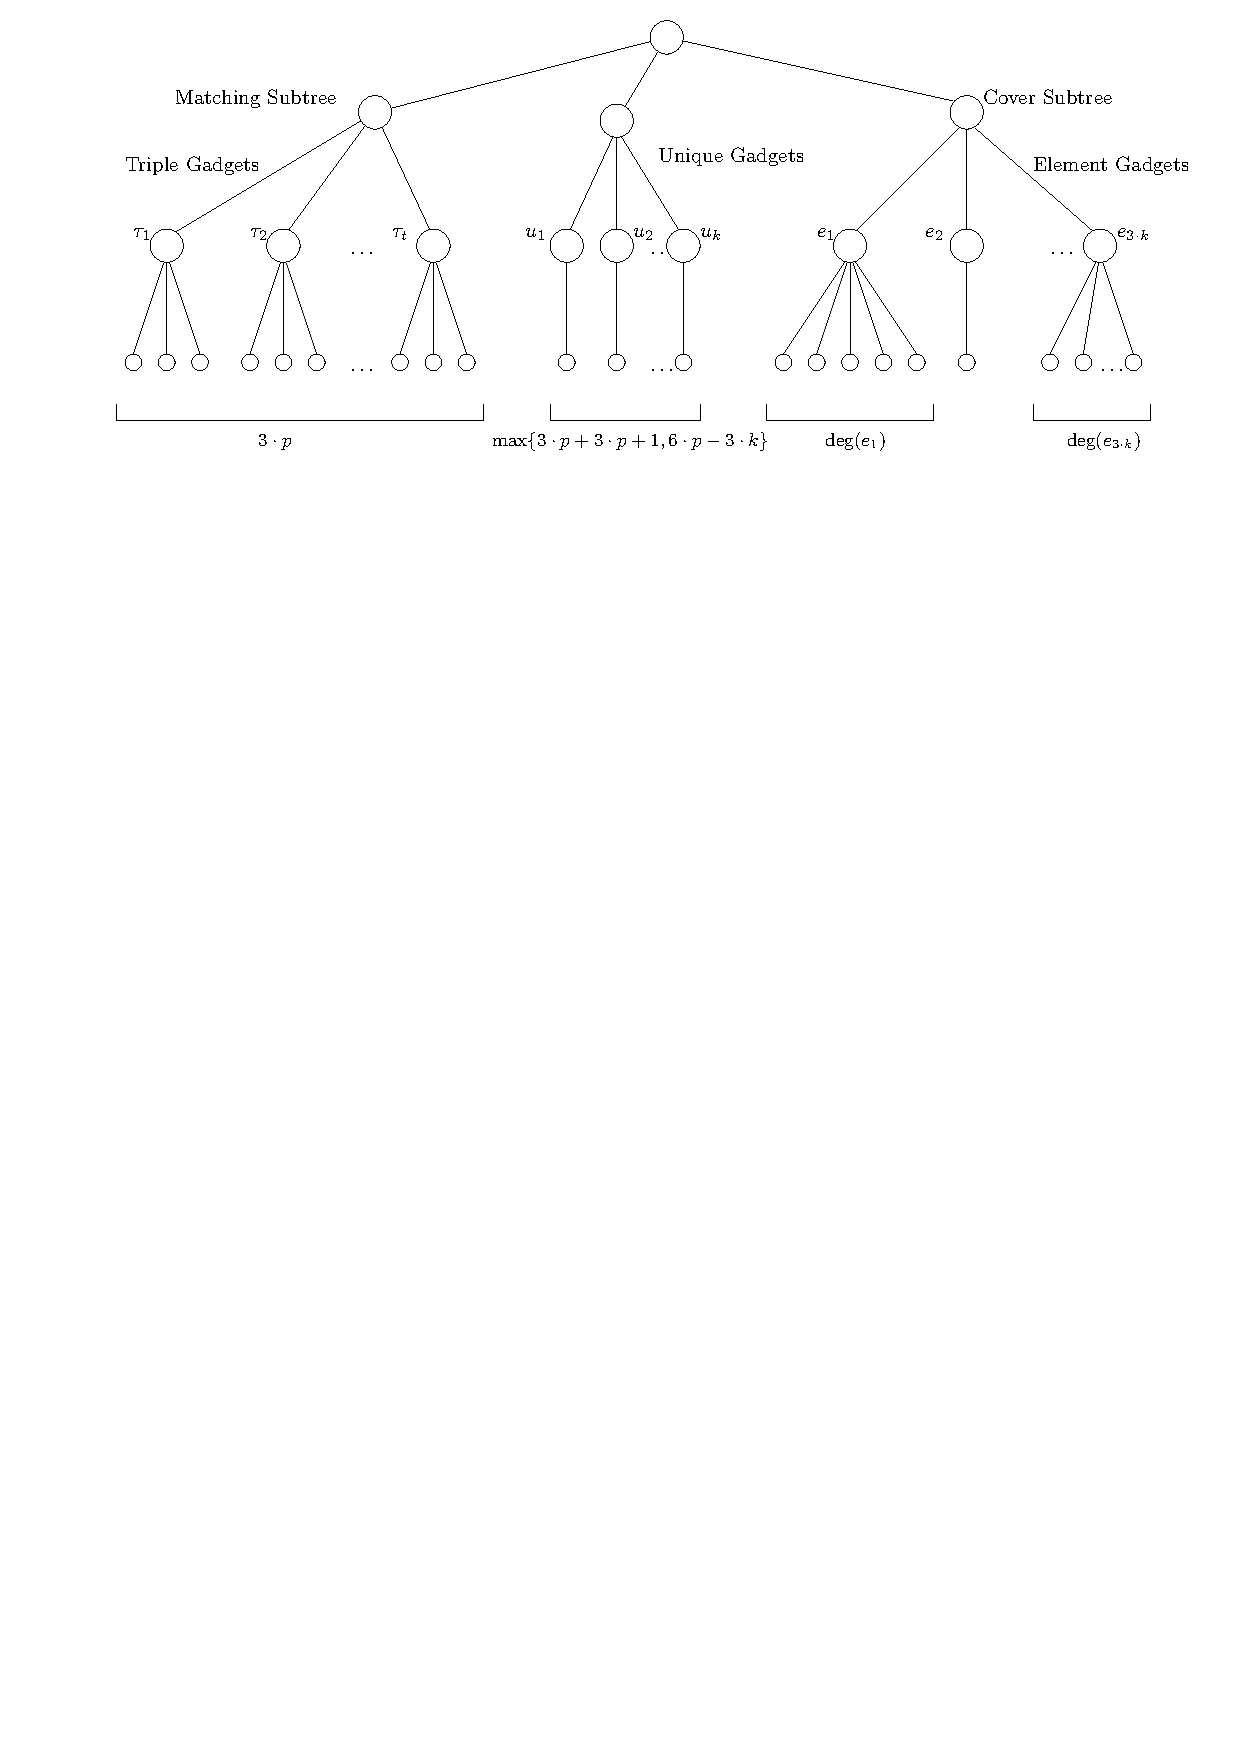
\includegraphics[width=0.9\columnwidth]{figs/static-mapping/overview2}
  \caption{Overview of the substrate network.}
  \label{fig:overview2}
\end{figure}


\emph{The substrate network.}
We construct the tree that has the following structure (see Figure~\ref{fig:overview2}):

\begin{enumerate}
  \item The physical network consists of three subtrees connected to
  the root: the {\MatchSubtree}, the {\CoverSubtree}, and a
  {\UnqSubtree}. In the {\MatchSubtree} we put $p$
  {\TripleGadgets}. The {\CoverSubtree} consist of~$k$ element gadgets.
  \item The {\UnqSubtree} consist of~$|U|$ leaves, and two middle nodes:
  a lower and an upper middle node. Note that this is different from the~$\RS(2)+\FP+\MA(4)$ variant NP-completeness proof, where {\UnqSubtree} was placed in the {\MatchSubtree}.
  \item The \TripleGadget: For each triple, we create a subtree
  consisisting of four vertices: three leaves and one triple root.  We
  attach the root of the triple to the root of the matching subtree.
  \item The \ElGadget: For each element~$e \in X\cup Y\cup Z$, we
  construct a subtree consisting of the root of the element (attached
  to the root of the cover subtree), and~$\deg(e)$ leaves.
\end{enumerate}

\emph{Chunk placement.}
The chunks are placed as follows:
\begin{enumerate}
  \item \emph{Chunks in the Matching Subtree:} In {\TripleGadget} of triple $t$ we put
  three replicas:
 ~$ch^{(1)}(t \cap X, t), ch^{(1)}(t \cap Y, t), ch^{(1)}(t \cap Z, t)$, one per each leaf.
  \item \emph{Chunks in the Unique Subtree:} We place replicas
 ~$U$ at the leaves of \UnqGadgets.
 \item \emph{Chunks in the Element Gadgets:} Consider the \ElGadget{} for the element $e \in X\cup Y\cup Z$.
 We place two types of replicas in the leaves of the gadget.
 We put replicas $ch^{(2)}(t, e)$ for each $t \in P_e$.
 In total, we place $\deg(e)$ replicas, one per each leaf of the gadget.
\end{enumerate}

\emph{Bandwidth constraints.} We use bandwidth constraints of the form
$\Band(k) := k\cdot(\numNodes - k)$, where $\Vms$ is the total number of nodes to be placed in the instance. Namely, we set the bandwidth
constraints of an uplink of an {\ElGadget} for each element~$e$ to 
$\Band(\deg(e)-1)$, the bandwidth of an uplink of a~$\MatchSubtree$ to 
$\Band(n)$, and an uplink of a~$\CoverSubtree$ to 
$\Band(\sum_e (\deg(e)-1)$.
Note that out of $\deg(e)$ leaves of the \ElGadget{} for element $e$, we allow to place $\deg(e)-1$ nodes.

\emph{The threshold value and other properties of the instance.} We set the
cost threshold for any solution to the following value:

%\begin{small}
\begin{align*}
  \Thr  & = 2\cdot \binom{3}{2}\cdot k & \mbox{(over 2 hops in the \MatchSubtree{})}\\
        & + 4 \cdot \binom{3\cdot k}{2} & \mbox{(over 4 hops in the \MatchSubtree{})}\\
        & + 4 \cdot \binom{u}{2} & \mbox{(over 4 hops in the \UnqGadgets{})}\\
        & + \sum_e 2\cdot\binom{\deg(e)-1}{2} & \mbox{(over 2 hops in the \CoverSubtree{})}\\
        & + 4\cdot \binom{\sum_e(\deg(e)-1)}{2} & \mbox{(over 4 hops in the \CoverSubtree{})}\\
        & + 6\cdot\binom{\Vms}{2} & \mbox{(over 6 hops)}
\end{align*}
%\end{small}

where $\Vms$ is the total number of nodes to be placed in the instance, and $u = |U|$.
  We
set~$\CostTrans$, the cost of chunk transportation to $\Thr+1$ (so that no chunk transportation happens in any feasible solution), 
$\CostCom = 1$, and we host only one node per machine. We set the
number of machines to place to:
$\numNodes := 3\cdot k + \sum_e (\deg(e)-1) + |U|$.
\\

\parag{Properties of the substrate network.}
\begin{lemma}
  Assume we have a~$\RS(2)+\FP+\NI+\BW$ variant instance~$I$ with a subtree
 ~$T'$ with~$l$ leaves and the bandwidth capacity on uplink of~$T'$ is
 ~$\Band(k)$. Assume that no chunk transportation is allowed
  ($\CostTrans = \infty$, so every node must be collocated with the
  chunk it processes in every feasible solution), and~$\CostCom = 1$.
  Then in any feasible solution the number $s$ of nodes placed in~$T'$ satisfies~$s \leq k \vee \Vms-s\leq k$, and~$s \leq l$.
  \label{lem:bandwidth1}
\end{lemma}

\begin{proof}
It holds that ~$s\leq l$ as we cannot place more nodes than leaves.
  The bandwidth allocation on the uplink of~$T'$ is
 ~$uplink(s,T) := s\cdot (\Vms - s)$, as no chunk transportation
  is allowed ($\CostTrans = \infty$), and every node in~$T'$ has to
  communicate over~$T'$'s uplink with nodes placed outside of
 ~$T'$. Therefore, in every feasible solution we have:
 ~$uplink(s, T') \leq \Band(k)$.  Let's define the remaining bandwidth
  on the uplink of $T'$~$\remainBw(s) := \Band(k)-uplink(s, T') = s^2 - s\cdot \Vms -
  k^2+k\cdot \Vms~$.
  Every feasible solution fulfills~$\remainBw(s) \geq 0$, which is true for
 ~$s \leq k \vee \Vms-s\leq k$ (follows from the properties of the
  quadratic function).
\end{proof}


Next, we show how to precisely control the number of nodes in the
constructed subtree.

\begin{obs}
  In every feasible solution we have exactly~$|U|$ nodes placed in a
  {\UnqSubtree} (no chunk transportation is allowed, and every chunk must be processed).
  \label{obs:unq-full}
\end{obs}


\begin{lemma}
  The following properties holds in $\SVCEMB$:
  \begin{enumerate}
    \item The number of nodes placed in a {\MatchSubtree} is
   ~$3\cdot k$.
    \item The number of nodes placed in a {\CoverSubtree} is
   ~$\sum_e(\deg(e)-1)$
  \end{enumerate}

  \label{lem:bandwidth2}
\end{lemma}

\begin{proof}
  From Observation~\ref{obs:unq-full} we know that we have~$|U|$ nodes
  in the {\UnqSubtree}. Let's refer to the number of nodes placed in
  a {\MatchSubtree} by~$M$, and to the number of nodes placed in
  {\CoverSubtree} by~$C$. By applying Lemma~\ref{lem:bandwidth1} to
  {\MatchSubtree}, we know that: $ M \leq 3\cdot k \vee M \geq \Vms - 3\cdot k$.
  We observe that~$\Vms - 3\cdot k$ is greater than the number of
  leaves in a {\MatchSubtree}.  By applying Lemma~\ref{lem:bandwidth1}
  to the {\CoverSubtree} we know that:~$ C \leq \sum_e(\deg(e)-1) \vee C$ $\geq \Vms - \sum_e(\deg(e)-1)$.
  We observe that~$\Vms - \sum_e(\deg(e)-1)$ is greater than the number
  of leaves in the {\CoverSubtree}.
  We also know that~$\Vms = |U| + C + M$. Therefore, by the pigeon-hole principle
 ~$C = \sum_e(\deg(e)-1)$ and~$M = 3\cdot k$.
\end{proof}


\begin{lemma}
  In the solution $\SVCEMB$, the number of nodes placed in Element Gadget of
  element~$e$ is~$\deg(e)-1$.
  \label{lem:bandwidth3}
\end{lemma}

\begin{proof}
  Let's call the number of nodes placed in the Element Gadget of
  element~$e$ the $x_e$.  From Lemma~\ref{lem:bandwidth1}, we know that
 ~$x_e \leq \deg(e) - 1 \vee x_e \geq \Vms - \deg(e) + 1$. We observe
  that~$\Vms - \deg(e) + 1$ is greater than the number of leaves of the
  gadget, which is~$\deg(e)$.  From Lemma~\ref{lem:bandwidth2}, we know
  that the number of nodes placed in the entire {\CoverSubtree} is
 ~$\sum_e (\deg(e)-1)$. Therefore, by the pigeon-hole principle, we have
  that~$x_e = \deg(e)-1$.
\end{proof}

From the above lemmas we know the precise number of nodes placed in
certain parts of the tree. Feasible solutions only differ in 
the choice of the~$\deg(e) - 1$ out of~$\deg(e)$ chunks
in each Element Gadget, and the placement of nodes in the
{\MatchSubtree}.



Similar in spirit to the NP-completeness proof of the~$\RS(2)+\MA(4)+\FP$ variant,
we call the {\TripleGadget} active if it contains exactly three nodes. 
Similarly, we call the {\TripleGadget} inactive if it
does not contain placed nodes, and \emph{partially active} if it
has one or two
placed nodes.

\begin{lemma}
  In $\SVCEMB$, we have exactly~$k$ active
  {\TripleGadgets}.
  \label{lem:full-or-empty}
\end{lemma}

\begin{proof}
  Since~$I$ is feasible, we know that it has a solution~$\Sol$ of
  cost~$\leq \Thr$.
  By Lemma~\ref{lem:bandwidth2}, we know that there are
  exactly~$3\cdot k$ placed nodes in the {\MatchSubtree}. Therefore, by
  the pigeon-hole principle, we know that we have at most~$k$
  active {\TripleGadgets}. It remains to show that there
  are no partially active {\TripleGadgets} in the solution of cost
 ~$\leq \Thr$.
  Using Lemma~\ref{lem:bandwidth3}, 
  we conclude that the communication cost of
  nodes in the {\CoverSubtree} is the same for every feasible solution
  (let's name that cost~$P$). We also know that the communication cost
  between nodes in {\CoverSubtree} and {\MatchSubtree} is the same for
  every feasible solution (let's name it~$Q$). Let's call the
  would-be cost of communication in the {\MatchSubtree}, if there were
  exactly~$k$ active gadgets,~$R$.
  The threshold value was chosen so that~$\Thr = P+Q+R$. If we have at least one partially active
  gadget, then the cost of communication in {\MatchSubtree} is greater
  than~$R$, because we increase the number of 4-hop communications by
  at least one per each partially active gadget in comparison to a solution
  where we have exactly~$k$ active gadgets.
\end{proof}

\parag{The reduction.}
Using the properties of the substrate network, we perform the reduction in the following way.

\begin{theorem}
 The $\RS(2)+\FP+\NI+\BW$ variant of the $\CTE$ problem is NP-hard.
\end{theorem}

\begin{proof}
  Fix an instance $\ITDPM$ of~$\TDPM$.
  We show that~$\IVCEMB$ has a solution of cost~$\leq \Thr$ if and only if~$\ITDPM \in \TDPM$ (there exists a perfect 3D matching in $\ITDPM$).


  Fix an instance~$\ITDPM$ of~$\TDPM$ and construct an instance~$\ICTE$
  of~$\RS(2)+\FP+\NI+\BW$ in the way described above.  We show that
 ~$\ICTE$ has solution of cost~$\leq \Thr$ if and only if~$I \in \TDPM$
  (there exists a perfect 3D matching).

  ($\Leftarrow$) Fix a feasible solution~$\STDPM$ for~$\ITDPM$ and
  produce a solution~$\SVCEMB$ to~$\IVCEMB$ in the way described in the construction section. We show that the cost of~$\SVCEMB$ is
  indeed~$\leq \Thr$.
  For each triple~from $P$ in~$\STDPM$, we put~$3$ nodes at
  leaves of triple gadgets corresponding to those triples.  In each
  element gadget (that corresponds to element~$e$), we put~$\deg(e)-1$
  nodes. In each element gadget there is only one leaf without the
  node placed in it: this node contains the chunk replica that is
  processed in the {\MatchSubtree}.
  It is easy to see that~$\SVCEMB$ has cost exactly~$\Thr$ and no
  bandwidth constraint is violated. Each chunk is processed.

  ($\Rightarrow$) Fix a feasible solution~$\SVCEMB$ for~$\IVCEMB$ and
  produce a solution~$\STDPM$ to~$\ITDPM$ by taking triples that correspond
  to active triple gadgets. Using Lemma~\ref{lem:full-or-empty}, we
  conclude that there are exactly~$k$ active triple gadgets. By
  feasibility of~$\STDPM$, we know that each chunk is
  processed. From Lemma~\ref{lem:bandwidth3}, we know that out
  of~$\deg(e)$ chunks that correspond to~$e\in X\cup Y\cup Z$,
  exactly one is processed in the {\MatchSubtree}, hence each
  element of~$X\cup Y\cup Z$ is matched.
\end{proof}


%%%%%%%%%%%%%%%%%%%%%%%%%%%%%%%%%%%%%
\section{Conclusions}\label{sec:conclusion-static}


In this chapter we have shown that despite the
multiple dimensions of flexibility in terms of chunk assignment and node placement, 
and despite the large scale of modern datacenters, 
many variants can be solved efficiently. However, we have also
shown that several embedding variants are NP-hard already in two-
and three-level trees---a practically relevant result given today's datacenter topologies~\cite{fattree}.


%\begin{table}
%\tiny
%\bgroup
%\def\arraystretch{1.5}
%\begin{small}
%\begin{tabular}{|l|l|p{6.5cm}|}
%\hline
%\multirow{3}{*}{NP-hard} & 5 combinations & \mbox{$\RS+\MA+\FP+\NI+\BW$}\\
%\cline{2-3}
% & 4 combinations &  \mbox{$\RS+\MA+\FP+\NI$}; \mbox{$\RS+\MA+\FP+\BW$};
%\mbox{$\RS+\FP+\NI+\BW$} \\ \cline{2-3}
% & 3 combinations &\mbox{$\RS+\MA+\FP$};~\mbox{$\RS+\FP+\NI$} \\
% \hline
% \hline
%\multirow{3}{*}{Flow} & 4 combinations & \mbox{$\RS+\MA+\NI+\BW$} \\ \cline{2-3}
% & 3 combinations & \mbox{$\RS+\NI+\BW$}; \mbox{$\RS+\MA+\BW$}    \\ \cline{2-3}
% & 2 combinations &$\RS+\BW$ \\
% \hline
% \hline
%\multirow{3}{*}{DP} & 4 combinations & \mbox{$\MA+\FP+\NI+\BW$} \\ \cline{2-3}
% & 3 combinations &   \mbox{$\MA+\FP+\NI$};
%\mbox{$\MA+\FP+\BW$}; \mbox{$\FP+\NI+\BW$} \\ \cline{2-3}
% & 2 combinations & \mbox{$\MA+\FP$};~\mbox{$\FP+\NI$}; \\
% \hline
% \hline
%\multirow{3}{*}{Matching} &3 combinations&
%\mbox{$\RS+\MA+\NI$};~\mbox{$\MA+\NI+\BW$}  \\
%\cline{2-3}
% & 2 combinations & \mbox{$\RS+\MA$};
%\mbox{$\RS+\NI$}; \mbox{$\MA+\NI$};
%\mbox{$\MA+\BW$}; \mbox{$\NI+\BW$} \\ \cline{2-3}
%& 1 combinations & \mbox{$\RS$}; \mbox{$\MA$};
%\mbox{$\NI$}; \mbox{$\BW$}\\
% \hline
% \hline
% \multirow{3}{*}{0 Cost} & 3 combinations & \mbox{$\RS+\FP+\BW$}\\
%\cline{2-3}
% & 2 combinations & \mbox{$\RS+\FP$}; \mbox{$\FP+\BW$}\\ \cline{2-3}
% & 1 combinations & \mbox{$\FP$}\\
% \hline
%\end{tabular}
%\end{small}
%\caption{
%Fastest algorithms for different respective problem variants.
%}
%\vspace{-2em}
%\label{tab:summary}
%\egroup
%\end{table}


Our results are summarized in
Figure~\ref{fig:venn_full}.
One interesting takeaway from this figure regards
the question which properties render the problem
NP-hard. For instance, we see that,~$\BW$
does not influence the hardness of any variant,
while~$\RS$ is crucial for NP-hardness.
$\MA$ only affects hardness if combined with~$\RS$.
$\NI$ is trivial without~$\FP$, and~$\FP$ requires
more sophisticated algorithms when combined with~$\NI$ or~$\MA$;
in combination with~$\RS$ and~$\MA$ or~$\NI$,~$\FP$ renders the
problem NP-hard.
